%rubber: module pdflatex

\documentclass[11pt,a4paper]{article}

\usepackage[sans]{tcc_doc} % SDP style file
\usepackage[english]{babel}
\usepackage{amssymb,amsmath} % for the math symbols
\usepackage{mdwlist}
\usepackage{geometry}
\usepackage{marginnote}
\usepackage{datetime}
\usepackage{graphicx}
\usepackage{verbatim}
\usepackage{mathtools}
\usepackage{hhtensor}
\usepackage{color}
\usepackage{txfonts}

%\usepackage{stylefiles/fmtcount}
\usepackage{natbib}

\graphicspath{ {images/} }

\usepackage[boxruled,linesnumbered]{algorithm2e}
\usepackage{fmtcount}


% TODO:
% 1. Check if all new symbols have been explained when used for the first
% time.
% 2. Check if all symbols are actually being used.
% 3. Check the symbol definitions: rates, numbers, etc. to use the same main letter
% 4. Is there a way to use proper referencing of applicable and reference
% documents?



%%%%%%%%% START OF USER SETTINGS %%%%%%%%%%%%%%%%%%

% Enter here some information needed to fill in the template Title to appear
% on the front pages (will be filled in via the \sdpfrontpage command)
\newcommand{\bigdoctitle}{Implementation of the Rau-Cornwell MSMFS algorithm \xspace}
% Title to go in the "Document Status Sheet" Document number
\newcommand{\docnr}{TCC-SDP-151123-2\xspace}
% Context
\newcommand{\context}{(SDP.PIP)}
% Revision
\newcommand{\revision}{2\xspace}
% Author(s)
\newcommand{\docauthor}{T.J.\ Cornwell\xspace}
% Lead author (goes in the footer)
\newcommand{\leadauthor}{T.J.\ Cornwell\xspace}
% Release date (YYYY-MM-DD)
\newcommand{\docudate}{\today\ \currenttime}
% Document classification
\newcommand{\classification}{Unrestricted}
% Status of the document (draft/final/etc.)
\newcommand{\docstatus}{Draft\xspace}

% The definitions below are used for the signature tables in the preamble of
% the document
\newcommand{\firstsigname}{Name 1 - to be filled in}
\newcommand{\firstsigdesignation}{Designation 1 - to be filled in}
\newcommand{\firstsigaffiliation}{Affiliation 1 - to be filled in}

\newcommand{\secondsigname}{Name 2 - to be filled in}
\newcommand{\secondsigdesignation}{Designation 2 - to be filled in}
\newcommand{\secondsigaffiliation}{Affiliation 2 - to be filled in}

% Table with version numbers
\newcommand{\versiontable}{
  \begin{tabularx}{\textwidth}{|X|X|X|X|}
    \hline
    \bf{Version} & {\bf Date of issue} & {\bf Prepared by} & {\bf Comments}\\
    \hline
  \end{tabularx}
}

%%%%%%%%%%%%% END OF USER SETTINGS %%%%%%%%%%%%%%%%%%%

% Table with signatures
\newcommand{\signaturetable}[3]{
  \begin{tabularx}{\textwidth}{|X|X|X|}
    \hline
    Name & Designation & Affilitation\\
    \hline
    {#1} & {#2} & {#3}\\
    \hline
    Signature \& Date: & & \\
    & & \\
    & & \\
    \hline
  \end{tabularx}
}



% Table with affiliations
\newcommand{\organisationtable}{
  \begin{center}
    \sffamily{\bf ORGANISATION DETAILS}\end{center}
  \begin{table}[htb]
    \centering
    \begin{tabular}[htb]{|l|l|}
      \hline
      Name & Science Data Processor Consortium\\
      \hline
    \end{tabular}
  \end{table}
}


%%%%%%%%%%%%%%%%%%%% START YOUR DOCUMENT HERE %%%%%%%%%%%%%%%%%

\newcommand{\subsubsubsection}[1]{\noindent{\bf{#1}}}

%%%% Please DO USE the symbol definitions listed below to preserve
%%%% consistency.

%%%% If you need a new symbol, please add it here. If really want to modify
%%%% one, do so, just take care to do a search-and-replace for the entire document
% Symbol definitions



\begin{document}

% load automatic pages
\tccfrontpage

\sdptableofcontents

% Add here the abbreviations used in your document
\sdplistofabbreviations
\begin{basedescript}{\desclabelstyle{\pushlabel}\desclabelwidth{6em}}
    \item[CDR] Critical Design Review \vspace{-0.2cm}
    \item[FFT] Fast Fourier Transform\vspace{-0.2cm}
    \item[FLOP] Floating Point Operations \vspace{-0.2cm}
    \item[FLOPS] Floating Point Operations per Second \vspace{-0.2cm}
    \item[FoV] Field of View\vspace{-0.2cm}
    \item[MS-MFS] Multi-Scale Multi-Frequency Synthesis\vspace{-0.2cm}
    \item[PSF] Point Spread Function \vspace{-0.2cm}
    \item[SDP] Scientific Data Processor\vspace{-0.2cm}
    \item[SKA] Square Kilometre Array\vspace{-0.2cm}
    \item[SKAO] SKA Organisation\vspace{-0.2cm}
%    \item[] \vspace{-0.2cm}
\end{basedescript} 

\newcommand{\nuno}{{\left(\frac{\nu}{\nu_0}\right)}}
\newcommand{\dnuno}{{\left(\frac{\nu-\nu_0}{\nu_0}\right)}}

\newcommand{\dg}{^\dag}
\newcommand{\X}{\vec{x}}
\newcommand{\Xd}{\vec{{x}^\dag}}
\newcommand{\B}{\vec{b}}
\newcommand{\Bd}{\vec{b^\dag}}
\newcommand{\V}{\vec{V}}
\newcommand{\Vd}{\vec{V^\dag}}
\newcommand{\A}{{\tens{A}{s}}}
\newcommand{\Ad}{{\tens{A^\dag}{s}}}
\newcommand{\F}{{\tens{F}{s}}}
\newcommand{\Fd}{{\tens{F^\dag}{s}}}
\newcommand{\He}{{\tens{H}{s}}}
\newcommand{\Sa}{{\tens{S}{s}}}
\newcommand{\Sd}{{\tens{S^\dag}{s}}}
\newcommand{\Sna}{\tens{{S_{\nu}}{s}}}
\newcommand{\Snd}{\tens{{S_{\nu}^\dag}{s}}}
\newcommand{\T}{{\tens{T}{s}}}
\newcommand{\W}{{\tens{W}{s}}}
\newcommand{\Wd}{{\tens{W^\dag}{s}}}
\newcommand{\Pb}{{\vec{P}}}

%\newcommand{\Wim}{{\tens{W^{im}}}}
%\newcommand{\Wimd}{{\tens{{W^{im}}^\dag}}}
%\newcommand{\Wnt}{{\tens{W^{\rm {mfs}}_t}}}
%\newcommand{\Wntd}{{\tens{{W^{\rm {mfs}}_t}^\dag}}}
%\newcommand{\Wnp}{{\tens{W^{\rm mfs}_p}}}
%\newcommand{\Wnpd}{{\tens{{W^{\rm mfs}_p}^\dag}}}
%\newcommand{\Wnq}{{\tens{W^{\rm mfs}_q}}}
%\newcommand{\Wnqd}{{\tens{{W^{\rm {mfs}}_q}^\dag}}}
%\newcommand{\Wimn}{{\tens{W^{im}_{\nu}}}}
%\newcommand{\Wimnd}{{\tens{{W^{im}_{\nu}}^\dag}}}

\newcommand{\Wim}{{{\W^{\rm im}}}}
\newcommand{\Wimd}{{{{\W^{\rm im}}^\dag}}}
\newcommand{\Wnt}{{{\W^{\rm {mfs}}_t}}}
\newcommand{\Wntd}{{{{\W^{\rm {mfs}}_t}^\dag}}}
\newcommand{\Wnp}{{{\W^{\rm mfs}_p}}}
\newcommand{\Wnpd}{{{{\W^{\rm mfs}_p}^\dag}}}
\newcommand{\Wnq}{{{\W^{\rm mfs}_q}}}
\newcommand{\Wnqd}{{{{\W^{\rm {mfs}}_q}^\dag}}}
\newcommand{\Wimn}{{{\W^{\rm im}_{\nu}}}}
\newcommand{\Wimnd}{{{{\W^{\rm im}_{\nu}}^\dag}}}

\newcommand{\wnt}{{w_{\nu}^t}}
\newcommand{\wnq}{{w_{\nu}^q}}
\newcommand{\wntq}{{w_{\nu}^{t+q}}}
%\newcommand{\Wntn}{{\tens{w^{\rm mfs}_{t,\nu}}}}
%\newcommand{\Wntnd}{{\tens{{w^{\rm mfs}_{t,\nu}}^\dag}}}
%\newcommand{\Wnpn}{{\tens{W^{\rm mfs}_{p,\nu}}}}
%\newcommand{\Wnpnd}{{\tens{{W^{\rm mfs}_{p,\nu}}^\dag}}}

\newcommand{\pd}{{\partial}}
\newcommand{\mi}{{m_{I}}}
\newcommand{\R}{{R}}
\newcommand{\Rd}{{R^\dag}}
\newcommand{\I}{{\vec{I}}}

\newcommand{\Nt}{N_{\rm t}}
\newcommand{\Ns}{N_{\rm s}}
\newcommand{\Nc}{N_{\rm c}}

% Add here the symbols used in your document
%\clearpage \sdplistofsymbols
%\begin{basedescript}{\desclabelstyle{\pushlabel}\desclabelwidth{6em}}
%\item[$\bytes$] Length of a complex number in bytes \vspace{-0.2cm}
%\item[$\cbytes$] Length of a complex number in bytes \vspace{-0.2cm}
%\item[$\rbytes$] Length of a real number in bytes \vspace{-0.2cm}
%\item[$\bl$] Baseline length / GPU memory bandwidth \vspace{-0.2cm}
%\item[$\maxbl$] Maximum baseline length \vspace{-0.2cm}
%\item[$\membw$] Memory bandwidth \vspace{-0.2cm}
%\item [$\pciebw$] PCI-e bandwidth \vspace{-0.2cm}
%\item[$\viscompr$] Compression factor of visibilities for grdding for facets
%  \textcolor{red}{This symbol is not used in the document, consider removing.}
%  \vspace{-0.2cm}
%\item[$\vism$] Matrix of observed visibilities \vspace{-0.2cm}
%\item[$\da$] Extent of aperture \vspace{-0.2cm}
%\item[$\ds$] Diameter of antennas/stations \vspace{-0.2cm}
%\item[$\reff$] Reference frequency\vspace{-0.2cm}
%\item[$\fcc$] Convolution kernel computational cost\vspace{-0.2cm}
%\item[$\fci$] Factor between bandwidth and FLOPS (bytes/operations)\vspace{-0.2cm}
%\item[$\fgrid$] Gridding cost\vspace{-0.2cm}
%\item[$\fpatch$] Fraction of the maximum baseline below which the $\uv$
%  coverage is almost filled\vspace{-0.2cm}
%\item[$\fpr$] Cost for phase rotation\vspace{-0.2cm}
%\item[$\gainm$] 2$\times$2 block diagonal matrix of complex
%  gains\vspace{-0.2cm}
%\item[$\modskyvism$] Matrix of model sky visibilities\vspace{-0.2cm}
%\item[$\skymodbufsize$] Size of the sky model buffer\vspace{-0.2cm}
%\item[$\visbufsize$] Size of the visibility buffer \vspace{-0.2cm}
%\item[$\visbufsizespec$] Size of the visibility buffer needed for spectral line processing\vspace{-0.2cm}
%\item[$\visbufsizecont$] Size of the visibility buffer needed for continuum imaging\vspace{-0.2cm}
%\item[$\bufsize$] Size of buffer \vspace{-0.2cm}
%\item[$\slowmemsize$] Size of slow working memory \vspace{-0.2cm}
%\item[$\cumemsize$] Size of working memory of compute unit \vspace{-0.2cm}
%\item[$\imgsize$] Size of image (bytes) \vspace{-0.2cm}
%\item[$\imgsizeoneax$] Image size along one axis \vspace{-0.2cm}
%\item[$\targgridsize$] Target grid size (per facet) \vspace{-0.2cm}
%\item[$\uvgridsize$] Size of the $\uv$ grid (bytes) \vspace{-0.2cm}
%\item[$\vissize$] Size of visibility data (bytes) \vspace{-0.2cm}
%\item[$\wgridsize$] Size of weight grid (bytes)\vspace{-0.2cm}
%\item[$\gridcachesize$] Cache size of gridding kernel \vspace{-0.2cm}
%\item[$\nbins$] Number of bins \vspace{-0.2cm}
%\item[$\ntel$] Number of antennas or stations in the array
%  \vspace{-0.2cm}
%\item[$\nateam$] Number of A-team sources \vspace{-0.2cm}
%\item[$\ngridpakern$] Number of grid points for A-kernel support (along one
%  axis) \vspace{-0.2cm}
%\item[$\naccvis$] Number of accesses per visibility \vspace{-0.2cm}
%\item[$\navg$] Number of averages\vspace{-0.2cm}
%\item[$\nbeam$] Number of beams simultaneously observed by the array
%  \vspace{-0.2cm}
%\item[$\nbits$] Number of bits\vspace{-0.2cm}
%\item[$\rma$] Number of flops in real multiply and add\vspace{-0.2cm}
%\item[$\cma$] Number of flops in complex multiply and add\vspace{-0.2cm}
%\item[$\nbl$] Number of baselines \vspace{-0.2cm}
%\item[$\nbyteacc$] Number of bytes per access \vspace{-0.2cm}
%\item[$\nbyte$] Number of bytes \vspace{-0.2cm}
%\item[$\nbyteperpix$] Number of bytes per pixel \vspace{-0.2cm}
%\item[$\nbytepervis$] Number of bytes per individual visibility 
%
%\item[$\nch$] Number of channels \vspace{-0.2cm}
%\item[$\ncompu$] Number of compute units \vspace{-0.2cm}
%\item[$\ndatait$] Number of data items required per source (e.g. position)\vspace{-0.2cm}
%\item[$\ngridp$] Number of grid points along one axis for the gridding
%  convolution function \vspace{-0.2cm}
%\item[$\nfch$] Number of frequency channels/sub-bands \vspace{-0.2cm}
%\item[$\nfchcorr$] Number of frequency channels output by the correlator
%  \vspace{-0.2cm}
%\item[$\nfchgrid$] Number of frequency channels to be gridded
%  \vspace{-0.2cm}
%\item[$\nfchdegrid$] Number of frequency channels to be de-gridded
%  \vspace{-0.2cm}
%\item[$\nfchout$] Number of frequency channels to be FFT-ed and reprojected
%  (output) or output from the CSP pulsar timing backend\vspace{-0.2cm}
%\item[$\nfchdist$] Minimum number of frequency channels to maintain distributability in the SDP
%\item[$\nfkernel$] Number of convolution kernels needed to cover frequency axis for a given baseline
%\item[$\nfacet$] Number of facets along one axis \vspace{-0.2cm}
%\item[$\nflop$] Number of floating point operations
%  \vspace{-0.2cm}
%\item[$\nflopsamp$] Number of floating point operations per sample
%  \vspace{-0.2cm}
%\item[$\nflopvis$] Number of floating point operations per visibility
%\item[$\npixgrid$] Number of pixels in the grid (i.e. the square of the linear
%  dimension) \vspace{-0.2cm}
%\item[$\ngridwkern$] Number of grid points for w-kernel support (along one
%  axis) \vspace{-0.2cm}
%\item[$\nit$] Number of iterations \vspace{-0.2cm}
%\item[$\nawkern$] Linear size of combined A and $\w$-kernels \vspace{-0.2cm}
%\item[$\nmaj$] Number of major CLEAN cycles (within each self-cal loop if appropriate) \vspace{-0.2cm}
%\item[$\nselfcal$] Number of self-calibration cycles \vspace{-0.2cm}
%\item[$\nmin$] Number of minor CLEAN cycles (within each major cycle loop if appropriate)\vspace{-0.2cm}
%\item[$\facgridoffdiagmuller$] Factor to account for gridding of off-diagonal
%  M\"uller terms \vspace{-0.2cm}
%\item[$\nops$] Number of operations \vspace{-0.2cm}
%\item[$\npatchpix$] Number of pixels of PSF to be used in minor cycle
%  decorrelation \vspace{-0.2cm}
%\item[$\npix$] Number of pixels along one axis of a grid\vspace{-0.2cm}
%\item[$\npixfacet$] Number of pixels on one side of a facet \vspace{-0.2cm}
%\item[$\npol$] Number of polarisation products \vspace{-0.2cm}
%\item[$\nsource$] Number of sources \vspace{-0.2cm}
%\item[$\ntslot$] Number of time slots \vspace{-0.2cm}
%\item[$\ntaylor$] Number of Taylor terms (in MS-MFS)\vspace{-0.2cm}
%\item[$\ntslotave$] Number of time slots that are averaged (in de-mixing)
%  \vspace{-0.2cm}
%\item[$\nvis$] Number of visibilities in an observation \vspace{-0.2cm}
%\item[$\qfacbw$] Quality factor \vspace{-0.2cm}
%\item[$\qfacreuse$] Factor to allow for the reuse of functions between
%  neighbouring frequency channels \vspace{-0.2cm}
%\item[$\qfacfov$] Quality factor defining how much bigger the diameter of the
%  field of view is than the first zero of the Airy function \vspace{-0.2cm}
%\item[$\facgridovers$] Gridding oversampling factor \vspace{-0.2cm}
%\item[$\facmsmf$] Factor to account for multiple subtractions (multi-frequency
%  multi-scale CLEAN\vspace{-0.2cm}
%\item[$\qfacbeamovers$] Quality factor defining the oversampling of the
%  synthesised beam \vspace{-0.2cm}
%\item[$\qfac$] Quality factor \vspace{-0.2cm}
%\item[$\Qkernel$] Convolution kernel quality factor, for kernel re-use in frequency
%\item[$\corrfacw$] Correction factor for w values (0 to 1) \vspace{-0.2cm}
%\item[$\earthrad$] Radius of the Earth ($6400\times 10^3$\,m) \vspace{-0.2cm}
%\item[$\covm$] Covariance matrix \vspace{-0.2cm}
%\item[$\covmfilt$] Filtered covariance matrix \vspace{-0.2cm}
%\item[$\comprate$] Compute rate (FLOPS) \vspace{-0.2cm}
%\item[$\compratespec$] Compute rate (FLOPS) for spectral line processing \vspace{-0.2cm}
%\item[$\compratecont$] Compute rate (FLOPS) for continuum imaging \vspace{-0.2cm}
%\item[$\compratefast$] Compute rate (FLOPS) for fast imaging \vspace{-0.2cm}
%\item[$\bwtoworkmem$] Bandwidth to working memory \vspace{-0.2cm}
%\item[$\maxmembw$] Maximum memory bandwidth of compute unit \vspace{-0.2cm}
%\item[$\peakflop$] Peak FLOPS of compute unit \vspace{-0.2cm}
%\item[$\maxiobwbuff$] Maximum I/O bandwidth of compute unit to buffer
%  \vspace{-0.2cm}
%\item[$\bwbuff$] Bandwidth to buffer \vspace{-0.2cm}
%\item[$\bwbuffcont$] Bandwidth to buffer for continuum imaging\vspace{-0.2cm}
%\item[$\bwbuffspec$] Bandwidth to buffer for spectral line processing\vspace{-0.2cm}
%\item[$\convkernflops$] Convolution kernel compute rate (FLOPS)\vspace{-0.2cm}
%\item[$\fftflops$] FFT compute rate (FLOPS)\vspace{-0.2cm}
%\item[$\griddingflops$] Gridding compute rate (FLOPS)\vspace{-0.2cm}
%\item[$\phaserotflops$] Phase rotation compute rate (FLOPS)\vspace{-0.2cm}
%\item[$\reprojflops$] Re-projection compute rate (FLOPS)\vspace{-0.2cm}
%\item[$\rcorr$] Correlator output rate\vspace{-0.2cm} TRY TO REMOVE
%\item[$\facetoverlap$]  ratio for linear size increase of facets to account for overlap, typically 1.2-1.5 \vspace{-0.2cm}
%\item[$\telsensit$] Telescope sensitivity \vspace{-0.2cm} TRY TO REMOVE
%\item[$\corrdumpt$] Correlator dump time (sec) \vspace{-0.2cm}
%\item[$\compt$] Computation time \vspace{-0.2cm}
%\item[$\gridkernupdate$] Update timescale for gridding kernel \vspace{-0.2cm}
%\item[$\lsmupdate$] Update timescale for the LSM \vspace{-0.2cm}
%\item[$\obst$] Observation time \vspace{-0.2cm}
%\item[$\snapshot$] Snapshot duration \vspace{-0.2cm}
%\item[$\minsnapshot$] Minimum duration of a snapshot in which w-correction is
%  not dominated by the Earth's curvature \vspace{-0.2cm}
%\item[$\optsnapshot$] Optimum snapshot duration (sec) \vspace{-0.2cm}
%\item[$\subint$] Sub-integration time\vspace{-0.2cm}
%\item[$\uvw$] Visibility coordinates \vspace{-0.2cm}
%\item [$\w$] Visibility $w$ coordinate \vspace{-0.2cm}
%\item[$\maxwdev$] Maximum deviation of the $w$ coordinate due to the Earth's
%  curvature \vspace{-0.2cm}
%\item[$\minwdev$] Minimum deviation of the $w$ coordinate due to the Earth's
%  curvature \vspace{-0.2cm}
%\item[$\spfiltm$] Spatial filter matrix \vspace{-0.2cm}
%\item[$\fres$] Frequency resolution \vspace{-0.2cm}
%\item[$\tres$] Time resolution (sec) \vspace{-0.2cm}
%\item[$\tressmear$]  Smearing Time resolution (sec)  \vspace{-0.2cm}
%\item[$\fracconvfuncamp$] Fraction of maximal amplitude of envelope of
%  convolution function \vspace{-0.2cm}
%\item[$\compeff$] Computational efficiency \vspace{-0.2cm}
%\item[$\fracfband$] Fraction of frequency band \vspace{-0.2cm}
%\item[$\beamsq$] Beam squint \vspace{-0.2cm}
%\item[$\fovdiam$] Angular diameter of the field of view (rad) \vspace{-0.2cm}
%\item[$\pixres$] Angular resolution of pixel size (rad) \vspace{-0.2cm}
%\item[$\beamdiam$] Angular diameter of the synthesised beam (rad)
%  \vspace{-0.2cm}
%\item[$\wavel$] Wavelength \vspace{-0.2cm}
%\item[$\maxwavel$] Maximum wavelength \vspace{-0.2cm}
%\item[$\minwavel$] Minimum wavelength \vspace{-0.2cm}
%\item[$\maxwavelsubb$] Maximum wavelength of an imaging sub-band (channels
%  over which image and pixel size are matched) \vspace{-0.2cm}
%\item[$\minwavelsubb$] Minimum wavelength of an imaging sub-band (channels
%  over which image and pixel size are matched) \vspace{-0.2cm}
%\item[$\earthrot$] Angular velocity of the Earth
%  ($7.27\times10^{-5}$\,rad/sec) \vspace{-0.2cm}
%\item[$\epsilonf$] Fraction of a uv cell that we allow uv track to move in time- or frequency- smearing-limited averaging \vspace{-0.2cm}
%\end{basedescript}

\sdplistoffigures

\sdplistoftables

% Add here the executive summary
\sdpsummary


\newpage

% Add to the table the list of applicable and reference documents (this is NOT
% meant for your usual bibiliography, only for SKA docs)
\sdpreferencedocs

\subsection*{Applicable Documents}

The following documents are applicable to the extent stated herein. In the
event of conflict between the contents of the applicable documents and this
document, \emph{the applicable documents} shall take precedence.

 \begin{center}
 \begin{tabularx}{\textwidth}{|l|X|}
     \hline
     \bf{Reference} & \bf{Reference}\\
     \bf{Number} & \\
     \hline
     {\bf [AD01]} & Dewdney, P. E. (2013). SKA1 System Baseline Design. SKA Office\\
     {\bf [AD02]} & McCool, R., Cornwell, T. (2013). Miscellaneous Corrections
     to the Baseline Design\\
     {\bf [AD03]} & SKA Phase 1 System (Level 1) Requirements Specification, T.Cornwell, SKA-OFF.SE.ARC-SKO-SRS-001\_2\\
     {\bf [AD04]} & PDR.01 SDP.ARCH document\\
     {\bf [AD05]} & SDP Costing spreadsheet\\
     {\bf [AD06]} & Cornwell, T.J. (2015). SKA1 Telescope Calibration
     Framework. SKA Office (draft version)\\
     {\bf [AD07]} & CSP--SDP ICD\\
     \hline
   \end{tabularx}
\end{center}

\clearpage
\subsection*{Reference Documents}

The following documents are referenced in this document. In the event of
conflict between the contents of the referenced documents and this document,
\emph{this document} shall take precedence.

 \begin{center}
 \begin{tabularx}{\textwidth}{|l|X|}
     \hline
     \bf{Reference} & \bf{Reference}\\
     \bf{Number} & \\
     \hline
   {\bf [RD01]} & SKA-TEL-SDP-0000041, F. Malan: iPython Performance Model Description\\
   {\bf [RD02]} & SKA-TEL-SDP-0000027, R. Nijboer: Pipelines Element Subsystem Design\\
   {\bf [RD03]} & SKA-TEL-SDP-0000038, R. Bolton: High Priority Science Objectives: Performance Analysis\\
   {\bf [RD04]} & SKA-TEL-SDP-0000028, A.-J. Boonstra: Ingest Pipeline\\
   {\bf [RD05]} & SKA-TEL-SDP-0000029, S. Salvini: Pipelines: Calibration\\
   {\bf [RD06]} & SKA-TEL-SDP-0000030, A. Scaife: Imaging Pipeline\\
   {\bf [RD07]} & SKA-TEL-SDP-0000031, M. Johnston-Hollitt: Science Analysis Pipeline\\
   {\bf [RD08]} & SKA-TEL-SDP-0000017, S. Wijnholds: Baseline-Dependent Averaging\\
   {\bf [RD09]} & SKA-TEL-SDP-0000058, S. Salvini: Fast Fourier Transforms\\
   {\bf [RD10]} & SKA-TEL-SDP-0000057, C. Skipper: Time and Channel Averaging\\
   {\bf [RD13]} & \url{http://www.astron.nl/casacore/trunk/casacore/doc/notes/229.html}\\
   {\bf [RD15]} & Imager.cc C++ source, CASA source code SVN revision 30821, \url{https://svn.cv.nrao.edu/svn/casa/trunk}\\ 
   {\bf [RD17]} & Parameterized deconvolution for wide-band radio synthesis imaging, Urvashi Rao Venkata, 2010, PhD thesis\\
   {\bf [RD18]} & S. Bhatnagar, T. J. (2008). Correcting direction-dependent gains in the deconvolution of radio interferometric images. A\&A, 419-429\\
   {\bf [RD22]} & Rik Jongerius, S. W. (2014). An End-to-End Computing Model for the Square Kilometre Array. IEEE Computer, volume 47, number 9\\
   {\bf [RD24]} & SDP Element Concept. Paul Alexander, Chris Broekema, Simon Ratcliffe, Rosie Bolton, Bojan Nikolic, 2013, SDP-PROP-DR-001-1 (part of SKA SDP Consortium proposal)\\
   {\bf [RD34]} & Cornwell, T. J. (2008). Multi-Scale CLEAN deconvolution of radio synthesis images. IEEE Journal of Selected Topics in Sig. Proc., 2, 793–801.\\
   {\bf [RD35]} & Conway, J. E., Cornwell, T. J., and Wilkinson, P. N. (1990). Multi-Frequency Synthesis - a New Technique in Radio Interferometric Imaging. Monthly Notices of the Royal Astronomical Society, 246, 490.\\  
   \hline
 \end{tabularx}
\end{center}







% The actual content goes here
\newpage
\section{Introduction}

\section{Purpose of the document}


The purpose of this document is to describe the Multi-Scale MultiFrequency Synthesis algorithm, the variant implementations in CASA and ASKAPsoft, and the scaling for insertion in the SDP Performance Model. We conclude with some recommendations.

\clearpage
\section{Scope of the document}

\clearpage
\section{Background}

MS-MFS was developed by Urvashi [RD17], melding together the concepts from multi-scale clean [RD34] and multi-frequency synthesis e.g. [RD35], with the goal of improving the reconstruction of sky brightness from radio interferometric data. The explicit model used for the sky brightness is a collection of blobs of varying scale sizes and strengths, each with spectral behaviour described by a power law expanded into a Taylor series.

The algorithm is an elaboration of the Multiscale CLEAN. It consists of two parts:
\begin{description}
\item[Major cycle] The image residuals for the current model are calculated by Fourier transform of the images constituting the power law expansion and degridding to obtain the predicted visibility, subtraction from the observed visibility, then gridding, and Fourier transformation to the image plane. There are two ways of performing this cycle depending on whether the Taylor series is calculated in image or uv space. Typically 5 - 10 major cycles are required.
\item[Minor cycle] The minor cycle is a greedy algorithm which identifies the dominant candidate scale and removes that using the appropriate PSF centered on that component. The minor cycle repeats this until convergence. Typically hundreds or thousands of iterations are required.
\end{description}

A canonical major/minor cycle algorithm is shown in Figure \ref{fig:majorminor}. The two functions Predict and MakeImage are sub-pipelines. ASKAPSoft and CASA both follow this form but with different ways of performing Predict (Figures \ref{fig:predictuv} and \ref{fig:predictimage}) and MakeImage (Figures \ref{fig:makeimageuv} and \ref{fig:makeimageimage})

\begin{figure}[htb]
  \centering
  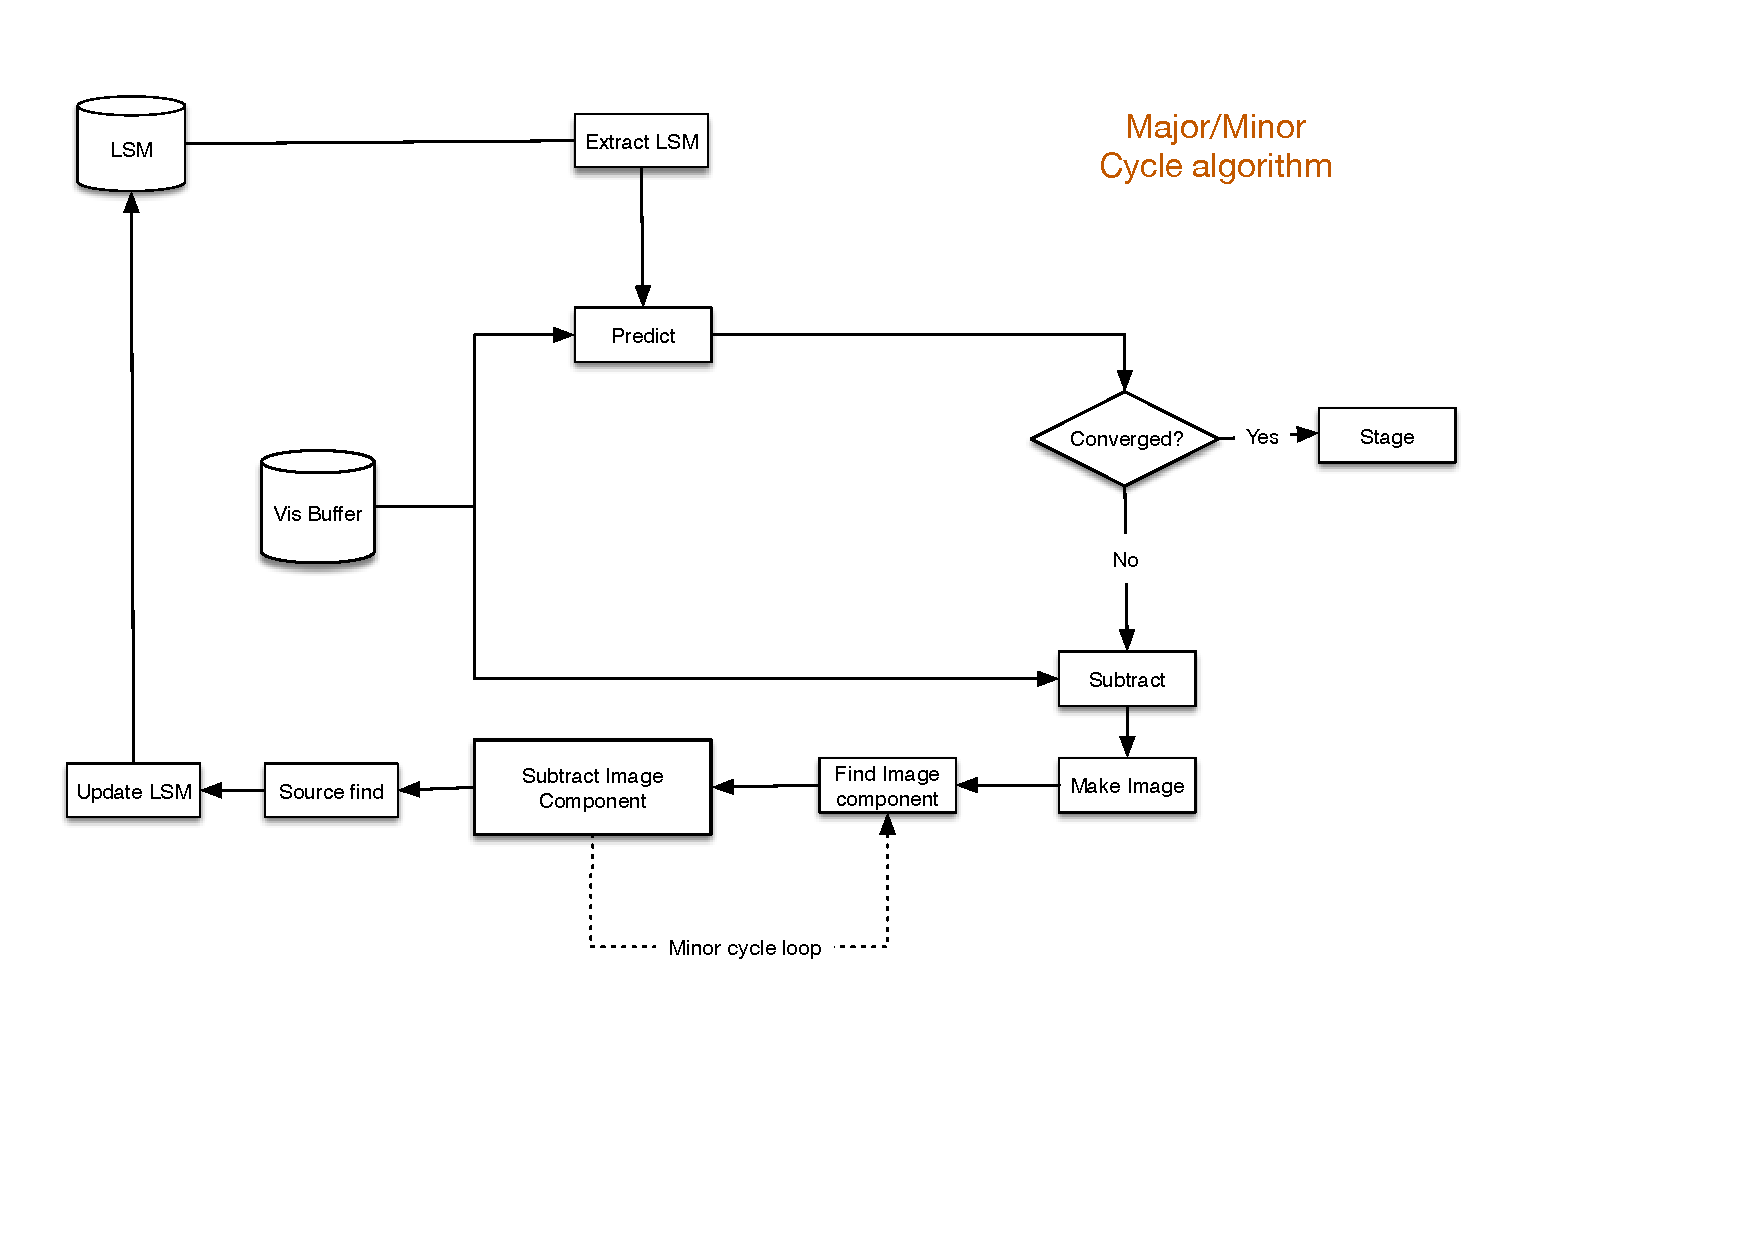
\includegraphics[width=\textwidth]{./MSMFS_MajorMinor.pdf}
  \caption{Structure of Major/Minor cycle algorithm}
  \label{fig:majorminor}
\end{figure}

The major cycle returns to the visibility data each iteration, whereas the minor cycle is entirely image-based.

MSMFS is relatively high in complexity because the usual CLEAN process is coupled over both scale (MSClean) and frequency or Taylor terms (MFS). The minor cycle must conduct a search in scale and Taylor term for each peak search. The major cycle requires calculation of the residual Taylor terms, which implies gridding and degridding all relevant frequency information. Memory use is high since a large number of images must be kept and updated as the iteration proceeds.



\clearpage
\section{Overview of MSMFS}
\label{sec:overview}

\subsection{Mathematical description}

In the Multi-Scale CLEAN [RD??], the sky is modelled as a set of blobs. Performing this decomposition using a gradient search algorithm is very demanding of resources. Instead, in MSCLEAN, a greedy algorithm obtained by generalising the CLEAN algorithm is used. The greedy algorithm locates the amplitude, scale and location of the blob by a straightforward search in the set of residual images, each smoothed with the appropriate blob. For each minor cycle this produces an amplitude, location, and scale. The smoothed residual images and model images are updated, and iteration proceeds.

\begin{equation}
\vec{I}^{model} = \sum_{s=0}^{N_s-1}  \vec{I}^{shp}_{s} \star \vec{I}^{sky,\delta}_s
\label{Eq:ms_model}
\end{equation}

where $N_s$ is the number of spatial scales used to construct the image, and
$\vec{I}^{sky,\delta}_{s}$ represents a collection of $\delta$-functions that describe the locations
and integrated amplitudes of flux components of scale $s$ in the image. $\vec{I}^{shp}_s$ is a tapered truncated parabola of width proportional to $s$.
The symbol $\star$ denotes convolution. 

The MSMFS algorithm decomposes the image into a set of $N_s$ blobs each with $N_t$ Taylor terms. 

\begin{eqnarray}
\label{eqn:mf_model}
\vec{I}^{model}_{\nu} = \sum_{t=0}^{N_t-1} \wnt \vec{I}^{sky}_{t} ~~~\mathrm{where}~~~ \wnt&=&\dnuno^t 
\end{eqnarray}

where $N_t$ is the order of the Taylor series expansion, and 
the $I^m_t$ represent multi-scale Taylor coefficient images.

Before performing any search, it is necessary to decouple the pixels in Taylor term space as well as possible. In practice, the Hessian (for each scale) for the peak of the PSF in Taylor term space is of modest size and can be inverted and used. The greedy algorithm then locates the scale and location in the reference-frequency image (as convolved with the set of scales). For each minor cycle this produces a location, scale, and values for all Taylor terms. The residual images and model images are updated, and iteration proceeds. The actual algorithm is shown in Figure \ref{fig:CASA}.


The image flux model at each frequency can be written as a linear sum of  
coefficient images at different spatial scales. 
\begin{equation}
\vec{I}^{model}_{\nu} = \sum_{t=0}^{N_t} \sum_{s=0}^{N_s} \wnt \left[ \vec{I}^{shp}_s \star \vec{I}^{sky}_\frac{s}{t}\right] ~~~~\mathrm{where}~~~\wnt = \dnuno^t 
\label{eqn:msmf_model}
\end{equation}

Here, $N_s$ is the number of discrete spatial scales used to represent the image and  
$N_t$ is the order of the series expansion of the spectrum. $\vec{I}^{sky}_\frac{s}{t}$ represents 
a collection of $\delta$-functions that describe the locations
and integrated amplitudes of flux components of scale $s$ in the image of the $t^{th}$ series 
coefficient. 

\clearpage
\section{CASA and ASKAPsoft implementations}

The MS-MFS algorithm as implemented in CASA shown in Algorithm \ref{CASA}. The ASKAPsoft version is shown in Algorithm \ref{ASKAP} with the variant lines in red.

%\begin{figure}[htb]
%  \centering
%  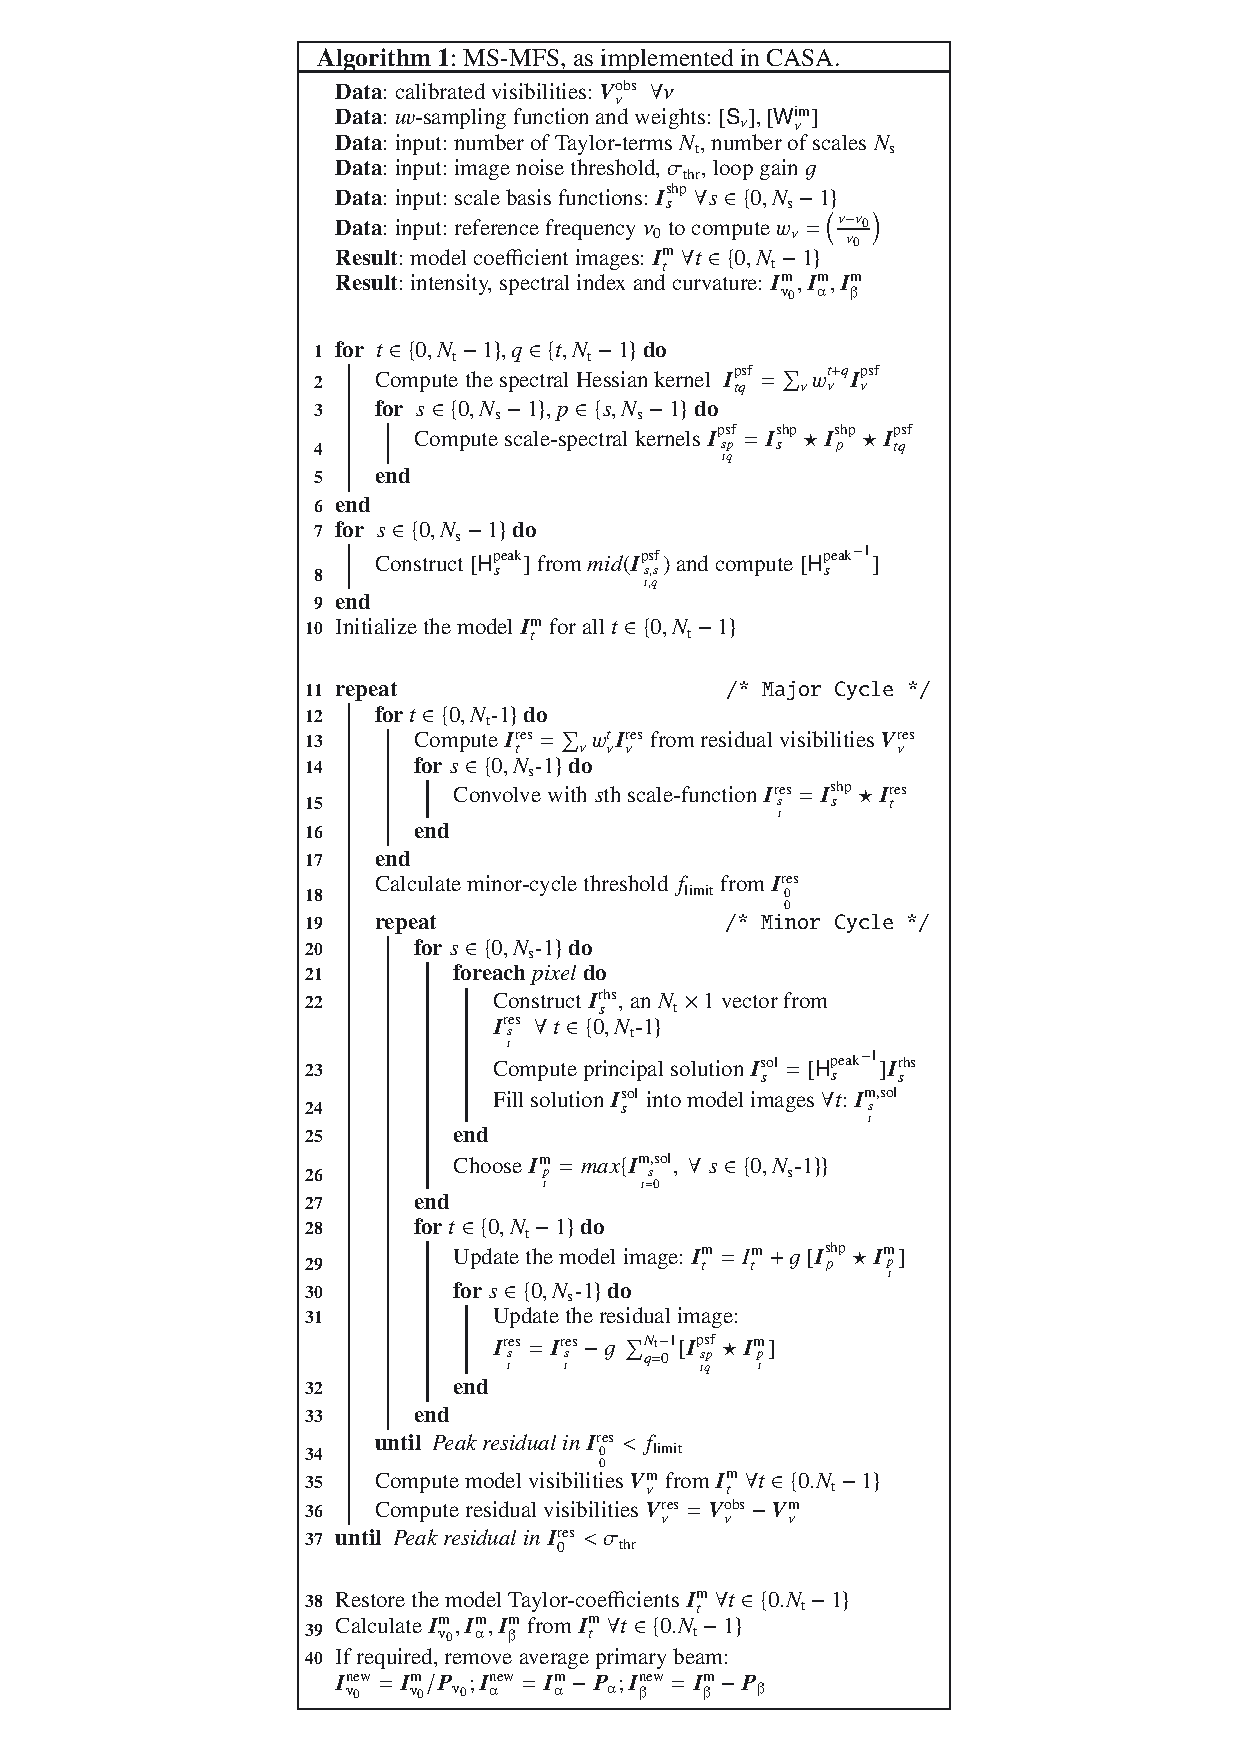
\includegraphics[width=\textwidth]{./algorithm.pdf}
%  \caption{The MSMFS algorithm as implemented in CASA [RD??]}
%  \label{fig:algoCASA}
%\end{figure}

\clearpage

\begin{algorithm}
\scriptsize
  \SetLine
  \linesnumbered
  \dontprintsemicolon
%  \SetKwRepeat{Repeat}{Repeat}{Until}
%  \SetKwFor{ForEach}{ForEach}{Do}{End}
%\KwData{ $\vec{V}^{corr}_{\nu}, \vec{I}^{\rm shp}_s~\forall~s\in\{0,\Ns $-$1\}, ~ [\Sna]~ \forall \nu$ }
%\KwResult{ $\vec{I}^{\rm psf}_{{sp}\atop{tq}},[{H^{\rm peak}_s}], \vec{I}^m_{\nu_0}, \vec{I}^{\alpha}, \vec{I}^{\beta}$ }
  \KwData{calibrated visibilities : $\vec{V}^{\rm obs}_{\nu}~~\forall \nu$}
  \KwData{$uv$-sampling function and weights : $[{\Sa}_{\nu}], [\Wimn]$}
  \KwData{input : number of Taylor-terms $\Nt $, number of scales $\Ns $}
  \KwData{input : image noise threshold, $\sigma_{\rm thr}$, loop gain $g$}
  \KwData{input : scale basis functions : $\I^{\rm shp}_s ~ \forall s\in\{0,\Ns -1\}$}
  \KwData{input : reference frequency $\nu_0$ to compute $w_{\nu}=\dnuno$}
  \KwResult{model coefficient images : $\I^{\rm m}_{t}~ \forall t\in\{0,\Nt -1\}$}
  \KwResult{intensity, spectral index and curvature : $\I^{\rm m}_{\nuup_0},\I^{\rm m}_{\alphaup},\I^{\rm m}_{\betaup}$}
 
%{Compute the dirty image $\vec{I}^{\rm dirty}$ and psf $\vec{I}^{\rm psf}$}\;
  \For{ $t \in \{0,\Nt -1\}, q \in \{t,\Nt -1\}$}
  {
        { Compute the spectral Hessian kernel } $\vec{I}^{\rm psf}_{tq} = \sum_{\nu} \wntq \vec{I}^{\rm psf}_{\nu}$\;
        \For{ $s \in \{0,\Ns -1\}, p \in \{s,\Ns -1\}$}
	{
		{Compute scale-spectral kernels} $\vec{I}^{\rm psf}_{{sp}\atop{tq}} = \vec{I}^{\rm shp}_s \star \vec{I}^{\rm shp}_p \star \vec{I}^{\rm psf}_{tq} $\;
	}
  }
  \For { $s \in \{0,\Ns -1\}$}
  {
     Construct scale-dependent Taylor space Hessian $[{\He^{\rm peak}_s}]$ from $mid(\I^{\rm psf}_{{s,s}\atop{t,q}})$ and compute $[{\He^{\rm peak}_s}^{-1}]$\;
  }
%%%%%%%%%%%%%%%%%%%%%%
%%%\vspace{0.5cm}
%%  \caption[MS-MFS CLEAN : Pre-Deconvolution Setup]
%%          {MS-MFS CLEAN : Pre-Deconvolution Setup}
%%\end{algorithm}
%%%\newpage
%%
%%\begin{algorithm}[\He]
%%  \SetLine
%%  \linesnumbered
%%  \dontprintsemicolon
%%%%%%%%%%%%%%%%%%%%%%%  
%%\KwData{ $\vec{V}^{corr}_{\nu}, \vec{I}^{\rm shp}_s, \vec{I}^{\rm psf}_{{sp}\atop{tq}},[{H^{\rm peak}_s}]~~~\forall~~s \in \{0,\Ns -1\}, p \in \{s,\Ns -1\}, \sigma_{thr}$ }
%%\KwResult{$I^{\rm m}_{q}~ \forall q \in \{0,\Nt -1\}$}
%%%%%%%%%%%%%%%%%%%%%  
  Initialize the model $\vec{I}^{\rm m}_t$ for all $t \in \{0,\Nt -1\}$\; % and compute $f_{sidelobe}$ \;
%  \vspace{0.5cm} 
  \Repeat (\tcc*[f]{Major Cycle}) { Peak residual in $\vec{I}^{\rm res}_0 < \sigma_{\rm thr}$ }
  {
    \For{$t \in \{0,\Nt $-$1\}$}
    {
      Compute $\vec{I}^{\rm res}_t = \sum_{\nu} \wnt \vec{I}^{\rm res}_{\nu}$ from frequency-weighted residual images $\I^{\rm res}_{\nu}$\;
      \For{$s \in \{0,\Ns $-$1\}$}
      {
	    Convolve with $s^{th}$ scale-function $\vec{I}^{\rm res}_{{s}\atop{t}} = \vec{I}^{\rm shp}_s \star \vec{I}^{\rm res}_t$
      }
    }
    Calculate minor-cycle threshold $f_{\rm limit}$ from $\vec{I}^{\rm res}_{{0}\atop{0}}$\;
%  \vspace{0.5cm} 
    \Repeat (\tcc*[f]{Minor Cycle}){ Peak residual in $\vec{I}^{\rm res}_{{0}\atop{0}} < f_{\rm limit} $ } 
    {
%     Compute $I^{\rm m}_q~\forall q\in \{0.\Nt -1\}$ and update $\vec{I}^{\rm res}_{{s},{t}}~\forall s,t$ (Algorithm \vref{MSMFS_2})\;
     \For{$s \in \{0,\Ns $-$1\}$}
     {
%      \uIf{Peak of $\vec{I}^{\rm res}_{s,0} > 10~\sigma_{thr} $}
%      {
       \ForEach{pixel}
       {
          Construct $\I^{\rm rhs}_s$, an $\Nt \times 1$ vector from $\I^{\rm res}_{{s}\atop{t}} ~~\forall ~ t \in \{0,\Nt $-$1\}$\;
          Compute principal solution $\I^{\rm sol}_s = [{\He^{\rm peak}_s}^{-1}] \I^{\rm rhs}_s$\;
          Fill solution $\I^{\rm sol}_s$ into model images $\forall t$ : $\I^{\rm m,sol}_{{s}\atop{t}}$
       }
 %     }
  %    \Else
%      {
 %      Find the location of the peak in $\vec{I}^{\rm res}_{s,0},~\forall~s\in\{0,\Ns $-$1\}$\;
 %      Construct $I^{\rm rhs}_s$, from $I^{\rm res}_{s,t}$ for the chosen $s$, at this location\;
 %      Compute $I^{sol} = [{H^{\rm peak}_s}^{-1}] I^{\rm rhs}_s$ at this location\;
 %     }
    }
       Choose $\I^{\rm m}_{{p}\atop{t}} = max\{\I^{\rm m,sol}_{{s}\atop{t=0}},~\forall~s\in\{0,\Ns $-$1\}\}$ \;
       \For{$t \in \{0,\Nt -1\}$}
       {
        Update the model image : $\I^{\rm m}_t = I^{\rm m}_t + g ~[ \I^{\rm shp}_{p} \star \I^{\rm m}_{{p}\atop{t}}]$ \;
        \For{$s \in \{0,\Ns $-$1\}$}
	{
          Update the residual image : $\I^{\rm res}_{{s}\atop{t}} = \I^{\rm res}_{{s}\atop{t}} - g ~\sum_{q=0}^{\Nt -1}[\I^{\rm psf}_{{sp}\atop{tq}} \star \I^{\rm m}_{{p}\atop{t}}]$\;
	}
       }
    }
%  \vspace{0.5cm} 
   Compute model visibilities $\V^{\rm m}_{\nu}$ from  $\I^{\rm m}_t~\forall t\in \{0.\Nt -1\}$\;
   Compute residual visibilities $\V^{\rm res}_{\nu} = \V^{\rm obs}_{\nu}-\V^{\rm m}_{\nu}$\;
  }
  \vspace{0.5cm} 
Restore the model Taylor-coefficients $\I^{\rm m}_t~\forall t\in \{0.\Nt -1\}$ \;
Calculate $\vec{I}^{\rm m}_{\nuup_0}, \vec{I}^{\rm m}_{\alphaup}, \vec{I}^{\rm m}_{\betaup}$ from $\I^{\rm m}_t~\forall t\in \{0.\Nt -1\}$\;
If required, remove average primary beam : $\vec{I}^{\rm new}_{\nuup_0}=\vec{I}^{\rm m}_{\nuup_0}/\vec{P}_{\nuup_0};  \vec{I}^{\rm new}_{\alphaup}=\vec{I}^{\rm m}_{\alphaup}-\vec{P}_{\alphaup};  \vec{I}^{\rm new}_{\betaup}=\vec{I}^{\rm m}_{\betaup}-\vec{P}_{\betaup}$\;
%\vspace{0.5cm}

  \caption[MS-MFS Algorithm]
         {MS-MFS, as implemented in CASA}\label{CASA}

\end{algorithm}

\begin{algorithm}
\scriptsize
  \SetLine
  \linesnumbered
  \dontprintsemicolon
%  \SetKwRepeat{Repeat}{Repeat}{Until}
%  \SetKwFor{ForEach}{ForEach}{Do}{End}
%\KwData{ $\vec{V}^{corr}_{\nu}, \vec{I}^{\rm shp}_s~\forall~s\in\{0,\Ns $-$1\}, ~ [\Sna]~ \forall \nu$ }
%\KwResult{ $\vec{I}^{\rm psf}_{{sp}\atop{tq}},[{H^{\rm peak}_s}], \vec{I}^m_{\nu_0}, \vec{I}^{\alpha}, \vec{I}^{\beta}$ }
  \KwData{calibrated visibilities : $\vec{V}^{\rm obs}_{\nu}~~\forall \nu$}
  \KwData{$uv$-sampling function and weights : $[{\Sa}_{\nu}], [\Wimn]$}
  \KwData{input : number of Taylor-terms $\Nt $, number of scales $\Ns $}
  \KwData{input : image noise threshold, $\sigma_{\rm thr}$, loop gain $g$}
  \KwData{input : scale basis functions : $\I^{\rm shp}_s ~ \forall s\in\{0,\Ns -1\}$}
  \KwData{input : reference frequency $\nu_0$ to compute $w_{\nu}=\dnuno$}
  \KwResult{model coefficient images : $\I^{\rm m}_{t}~ \forall t\in\{0,\Nt -1\}$}
  \KwResult{intensity, spectral index and curvature : $\I^{\rm m}_{\nuup_0},\I^{\rm m}_{\alphaup},\I^{\rm m}_{\betaup}$}
 
%{Compute the dirty image $\vec{I}^{\rm dirty}$ and psf $\vec{I}^{\rm psf}$}\;
  \For{ $t \in \{0,\Nt -1\}, q \in \{t,\Nt -1\}$}
  {
{\color{red}        { Compute the spectral Hessian kernel $\vec{I}^{\rm psf}_{tq}$ from transform of frequency weight sampling } $\sum_{\nu} \wntq \Sa_{\nu}$\;}
        \For{ $s \in \{0,\Ns -1\}, p \in \{s,\Ns -1\}$}
	{
		{Compute scale-spectral kernels} $\vec{I}^{\rm psf}_{{sp}\atop{tq}} = \vec{I}^{\rm shp}_s \star \vec{I}^{\rm shp}_p \star \vec{I}^{\rm psf}_{tq} $\;
	}
  }
  \For { $s \in \{0,\Ns -1\}$}
  {
     Construct scale-dependent Taylor space Hessian $[{\He^{\rm peak}_s}]$ from $mid(\I^{\rm psf}_{{s,s}\atop{t,q}})$ and compute $[{\He^{\rm peak}_s}^{-1}]$\;
  }
%%%%%%%%%%%%%%%%%%%%%%
%%%\vspace{0.5cm}
%%  \caption[MS-MFS CLEAN : Pre-Deconvolution Setup]
%%          {MS-MFS CLEAN : Pre-Deconvolution Setup}
%%\end{algorithm}
%%%\newpage
%%
%%\begin{algorithm}[\He]
%%  \SetLine
%%  \linesnumbered
%%  \dontprintsemicolon
%%%%%%%%%%%%%%%%%%%%%%%  
%%\KwData{ $\vec{V}^{corr}_{\nu}, \vec{I}^{\rm shp}_s, \vec{I}^{\rm psf}_{{sp}\atop{tq}},[{H^{\rm peak}_s}]~~~\forall~~s \in \{0,\Ns -1\}, p \in \{s,\Ns -1\}, \sigma_{thr}$ }
%%\KwResult{$I^{\rm m}_{q}~ \forall q \in \{0,\Nt -1\}$}
%%%%%%%%%%%%%%%%%%%%%  
  Initialize the model $\vec{I}^{\rm m}_t$ for all $t \in \{0,\Nt -1\}$\; % and compute $f_{sidelobe}$ \; 
  \Repeat (\tcc*[f]{Major Cycle}) { Peak residual in $\vec{I}^{\rm res}_0 < \sigma_{\rm thr}$ }
  {
    \For{$t \in \{0,\Nt $-$1\}$}
    {
{\color{red}      Compute $\vec{I}^{\rm res}_t = \sum_{\nu} \wnt \vec{I}^{\rm res}_{\nu}$ from frequency-weighted residual visibilities $\V^{\rm res}_{\nu}$\;}
      \For{$s \in \{0,\Ns $-$1\}$}
      {
	    Convolve with $s^{th}$ scale-function $\vec{I}^{\rm res}_{{s}\atop{t}} = \vec{I}^{\rm shp}_s \star \vec{I}^{\rm res}_t$
      }
    }
    Calculate minor-cycle threshold $f_{\rm limit}$ from $\vec{I}^{\rm res}_{{0}\atop{0}}$\;
%  \vspace{0.5cm} 
    \Repeat (\tcc*[f]{Minor Cycle}){ Peak residual in $\vec{I}^{\rm res}_{{0}\atop{0}} < f_{\rm limit} $ } 
    {
%     Compute $I^{\rm m}_q~\forall q\in \{0.\Nt -1\}$ and update $\vec{I}^{\rm res}_{{s},{t}}~\forall s,t$ (Algorithm \vref{MSMFS_2})\;
     \For{$s \in \{0,\Ns $-$1\}$}
     {
%      \uIf{Peak of $\vec{I}^{\rm res}_{s,0} > 10~\sigma_{thr} $}
%      {
       \ForEach{pixel}
       {
          Construct $\I^{\rm rhs}_s$, an $\Nt \times 1$ vector from $\I^{\rm res}_{{s}\atop{t}} ~~\forall ~ t \in \{0,\Nt $-$1\}$\;
          Compute principal solution $\I^{\rm sol}_s = [{\He^{\rm peak}_s}^{-1}] \I^{\rm rhs}_s$\;
          Fill solution $\I^{\rm sol}_s$ into model images $\forall t$ : $\I^{\rm m,sol}_{{s}\atop{t}}$
       }
 %     }
  %    \Else
%      {
 %      Find the location of the peak in $\vec{I}^{\rm res}_{s,0},~\forall~s\in\{0,\Ns $-$1\}$\;
 %      Construct $I^{\rm rhs}_s$, from $I^{\rm res}_{s,t}$ for the chosen $s$, at this location\;
 %      Compute $I^{sol} = [{H^{\rm peak}_s}^{-1}] I^{\rm rhs}_s$ at this location\;
 %     }
     }
     Choose $\I^{\rm m}_{{p}\atop{t}} = max\{\I^{\rm m,sol}_{{s}\atop{t=0}},~\forall~s\in\{0,\Ns $-$1\}\}$ \;
       \For{$t \in \{0,\Nt -1\}$}
       {
        Update the model image : $\I^{\rm m}_t = I^{\rm m}_t + g ~[ \I^{\rm shp}_{p} \star \I^{\rm m}_{{p}\atop{t}}]$ \;
        \For{$s \in \{0,\Ns $-$1\}$}
	{
          Update the residual image : $\I^{\rm res}_{{s}\atop{t}} = \I^{\rm res}_{{s}\atop{t}} - g ~\sum_{q=0}^{\Nt -1}[\I^{\rm psf}_{{sp}\atop{tq}} \star \I^{\rm m}_{{p}\atop{t}}]$\;
	}
       }
    }
%  \vspace{0.5cm} 
   {\color{red} Compute model visibilities $\V^{\rm m}_{\nu}$ from  $\V^{\rm m}_t~\forall t\in \{0.\Nt -1\}$}\;
   Compute residual visibilities $\V^{\rm res}_{\nu} = \V^{\rm obs}_{\nu}-\V^{\rm m}_{\nu}$\;
  } 
Restore the model Taylor-coefficients $\I^{\rm m}_t~\forall t\in \{0.\Nt -1\}$ \;
Calculate $\vec{I}^{\rm m}_{\nuup_0}, \vec{I}^{\rm m}_{\alphaup}, \vec{I}^{\rm m}_{\betaup}$ from $\I^{\rm m}_t~\forall t\in \{0.\Nt -1\}$\;
If required, remove average primary beam : $\vec{I}^{\rm new}_{\nuup_0}=\vec{I}^{\rm m}_{\nuup_0}/\vec{P}_{\nuup_0};  \vec{I}^{\rm new}_{\alphaup}=\vec{I}^{\rm m}_{\alphaup}-\vec{P}_{\alphaup};  \vec{I}^{\rm new}_{\betaup}=\vec{I}^{\rm m}_{\betaup}-\vec{P}_{\betaup}$\;
%\vspace{0.5cm}

  \caption[MS-MFS Algorithm]
         {MS-MFS, as implemented in ASKAPsoft: {\color{red} red denotes difference from CASA}}\label{ASKAP}

\end{algorithm}

We can relate these back to the graphical form Figure \ref{fig:majorminor} by introducing variant sub pipelines for Predict and MakeImage. These are graphically shown in Figures \ref{fig:predictuv} to \ref{fig:makeimageimage}: 

\begin{figure}[htb]
  \centering
  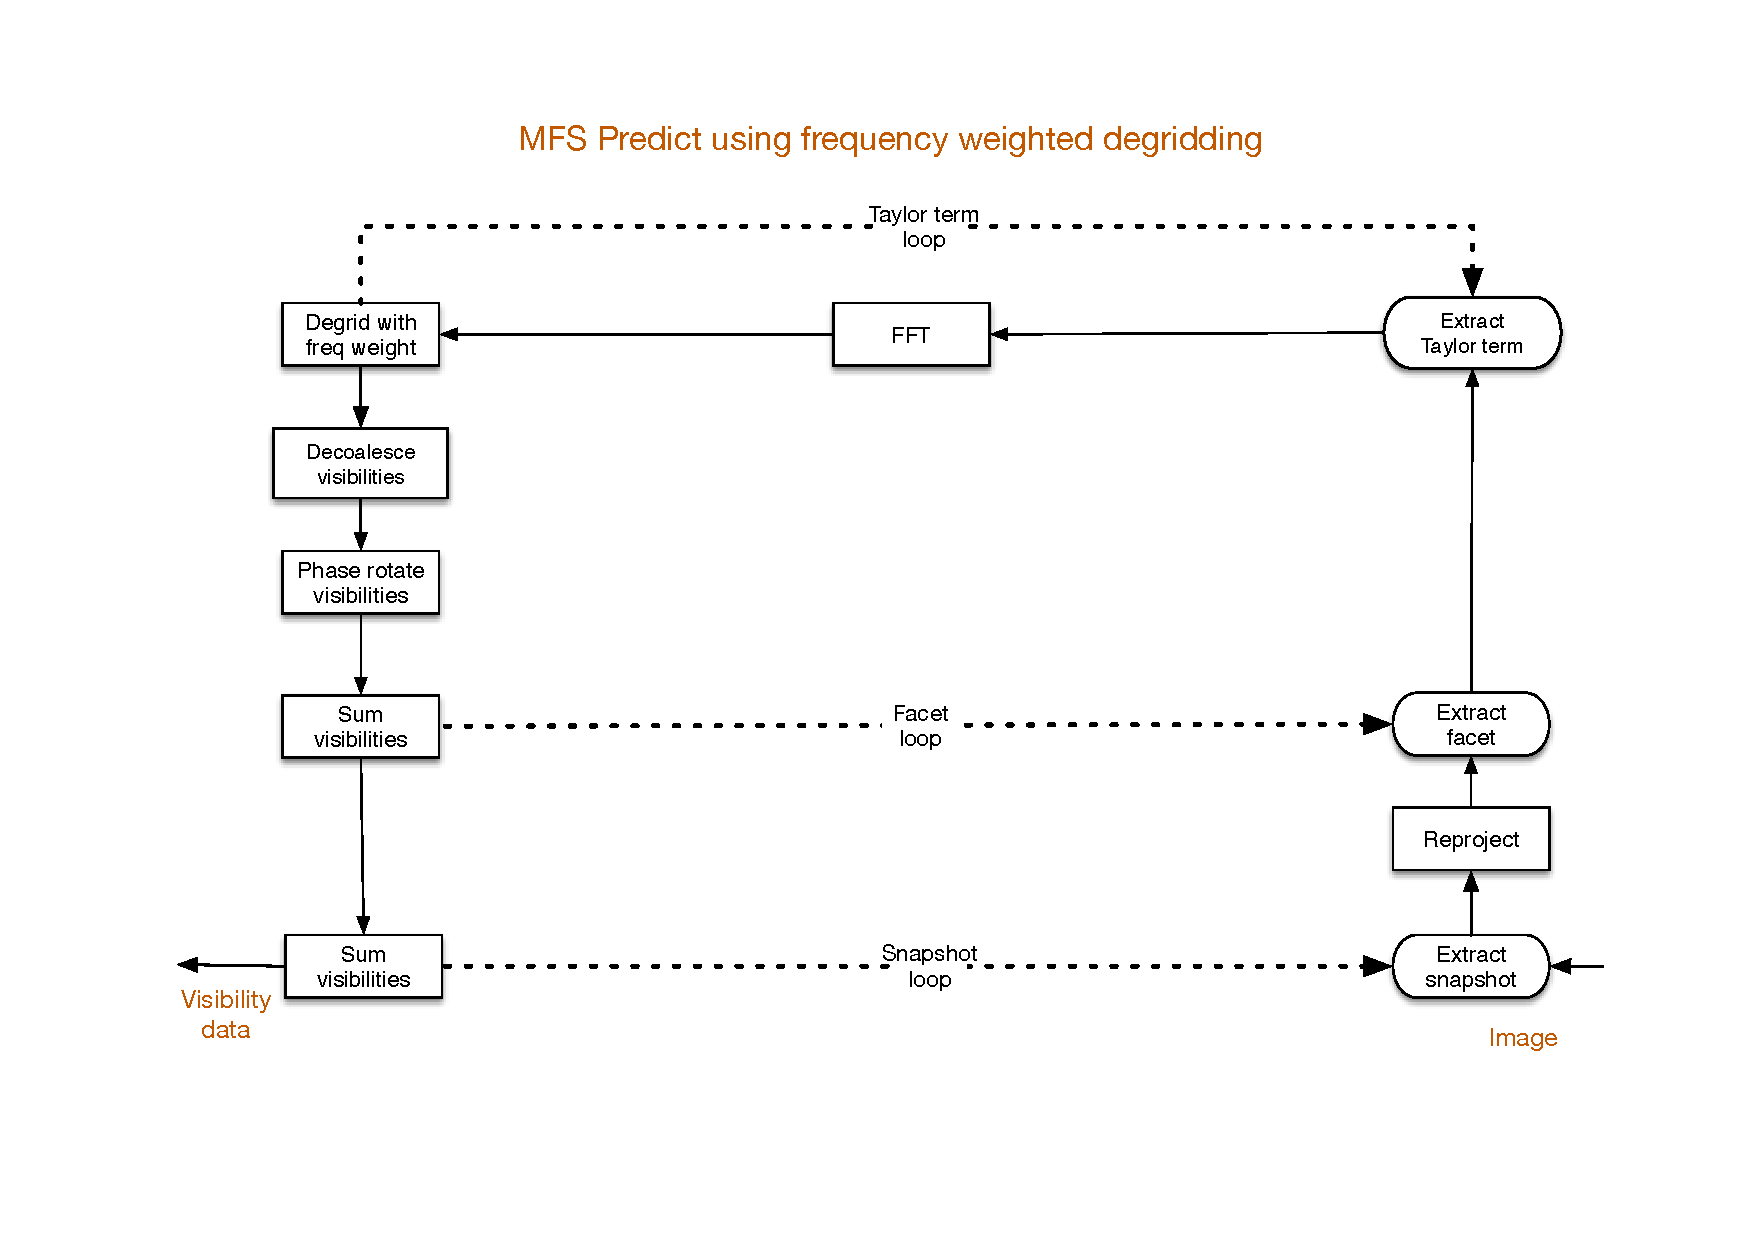
\includegraphics[width=\textwidth]{./MSMFS_Predict_UV.pdf}
  \caption{Structure of UV-weighting Predict, as used in ASKAPsoft. }
  \label{fig:predictuv}
\end{figure}

\begin{figure}[htb]
  \centering
  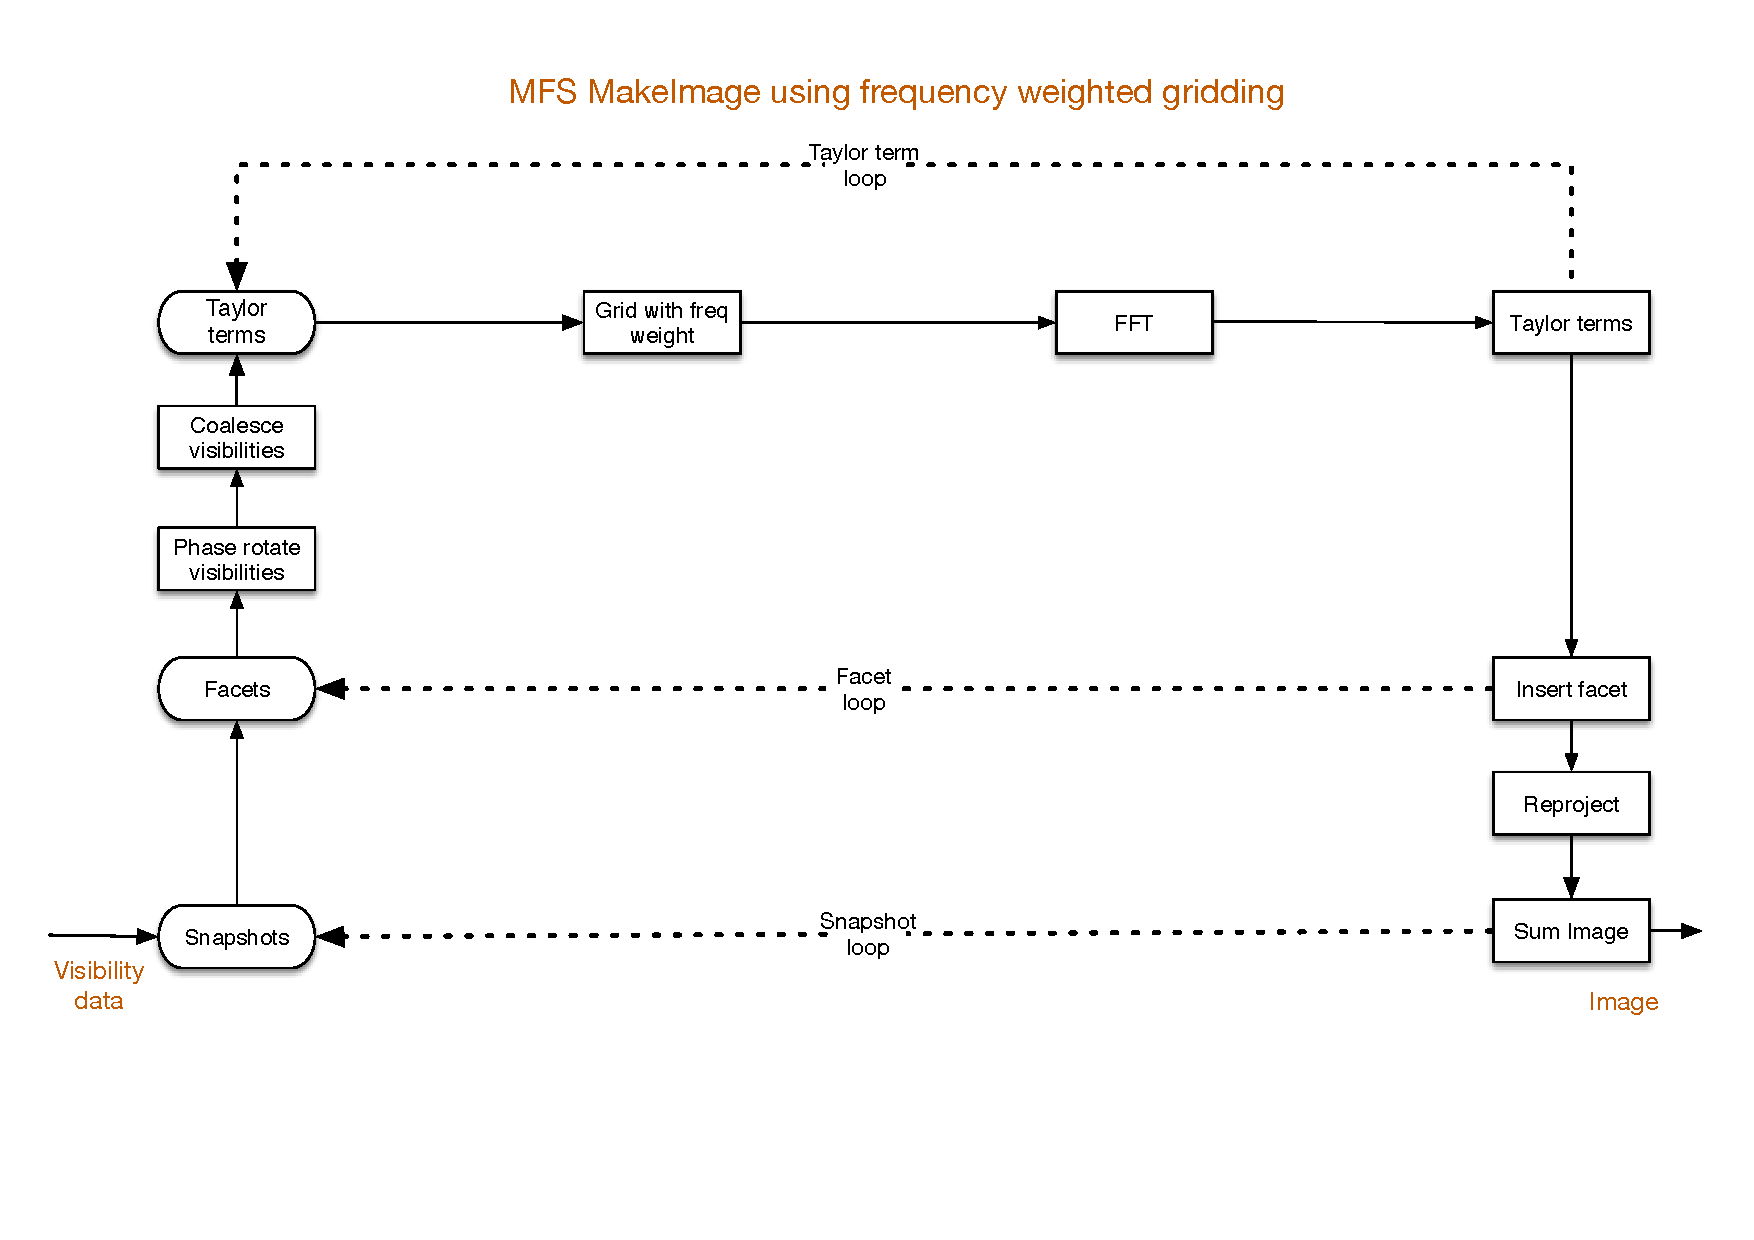
\includegraphics[width=\textwidth]{./MSMFS_MakeImage_UV.pdf}
  \caption{Structure of UV-weighting MakeImage, as used in ASKAPsoft. Note that the three loops (denoted by the rectangle with curved ends) can be permutated at will.}
  \label{fig:predictimage}
\end{figure}


\begin{figure}[htb]
  \centering
  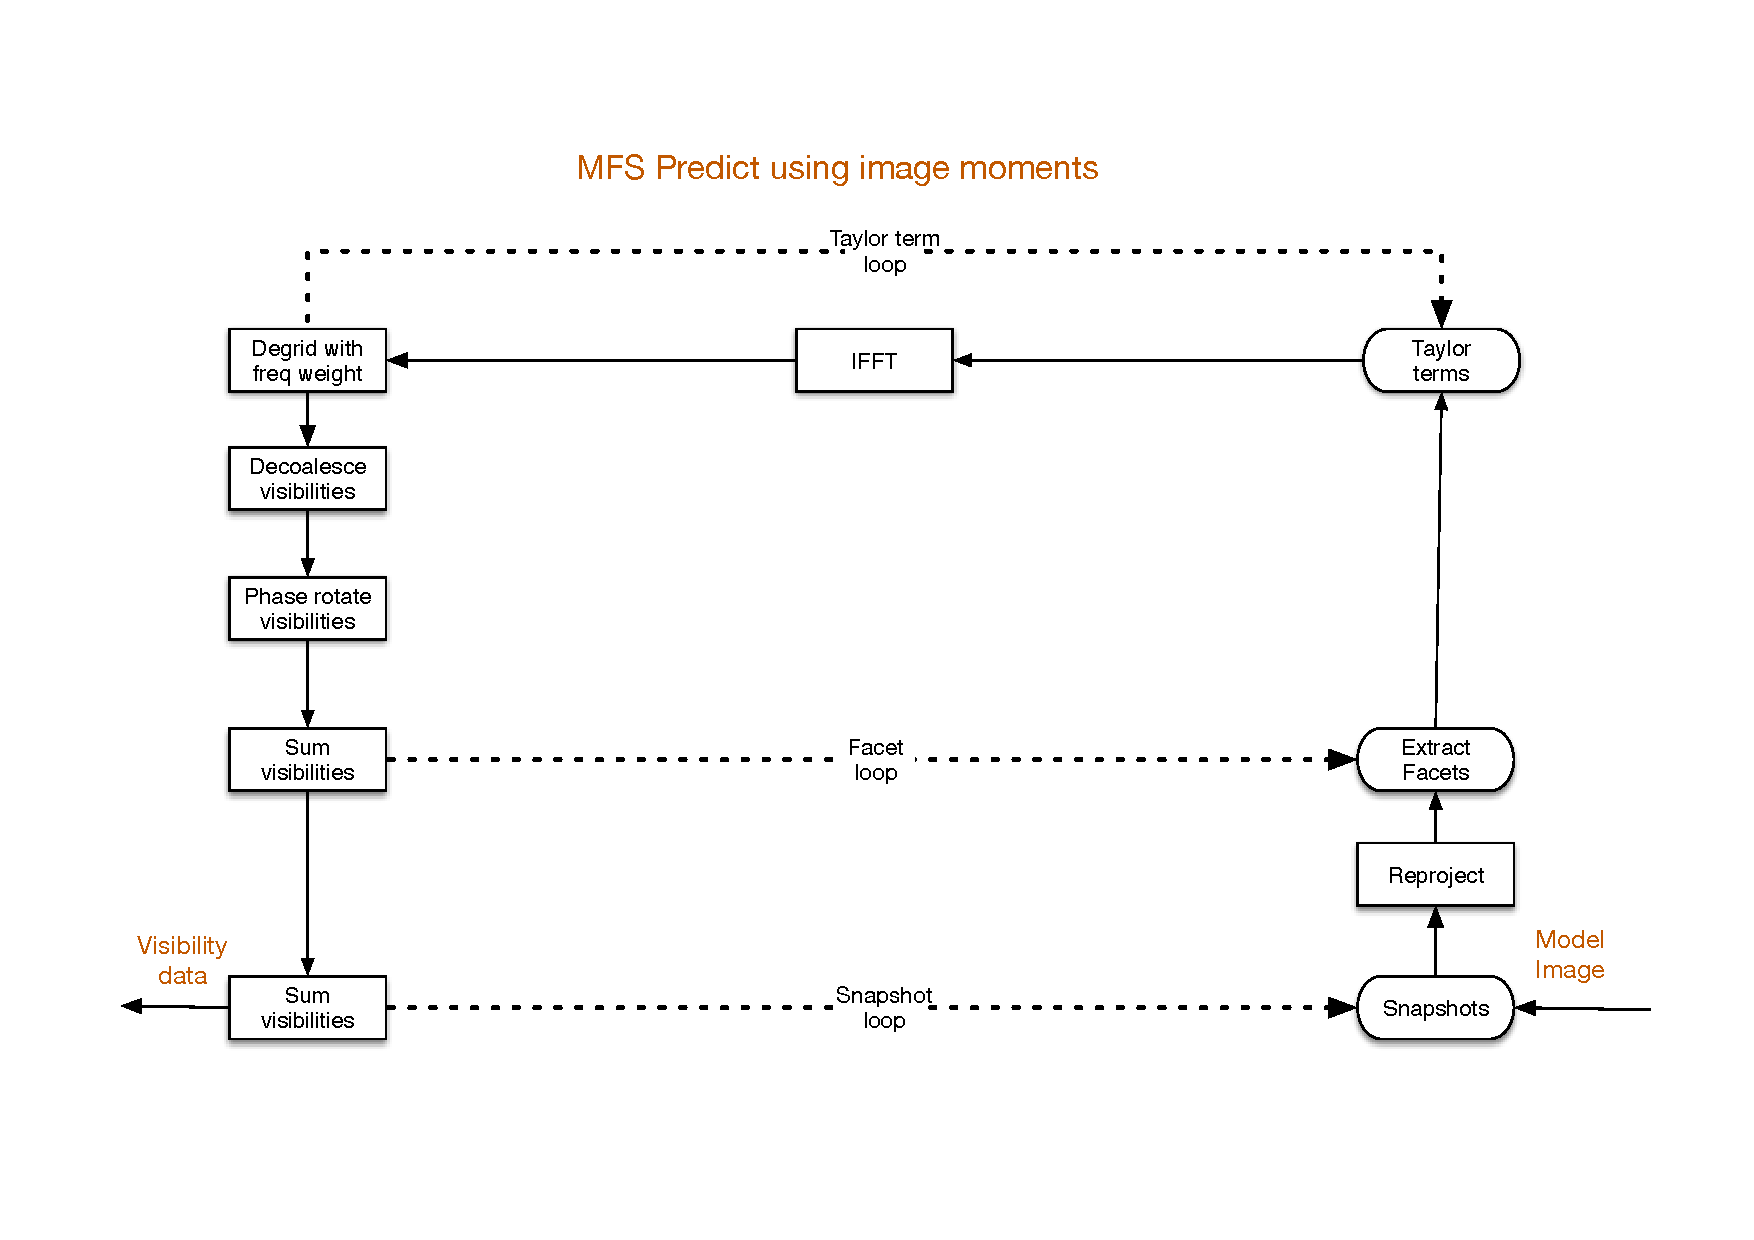
\includegraphics[width=\textwidth]{./MSMFS_Predict_Image.pdf}
  \caption{Structure of Image plane-weighting Predict, as used in CASA. Note that the three loops (denoted by the rectangle with curved ends) can be permutated at will.}
  \label{fig:makeimageuv}
\end{figure}


\begin{figure}[htb]
  \centering
  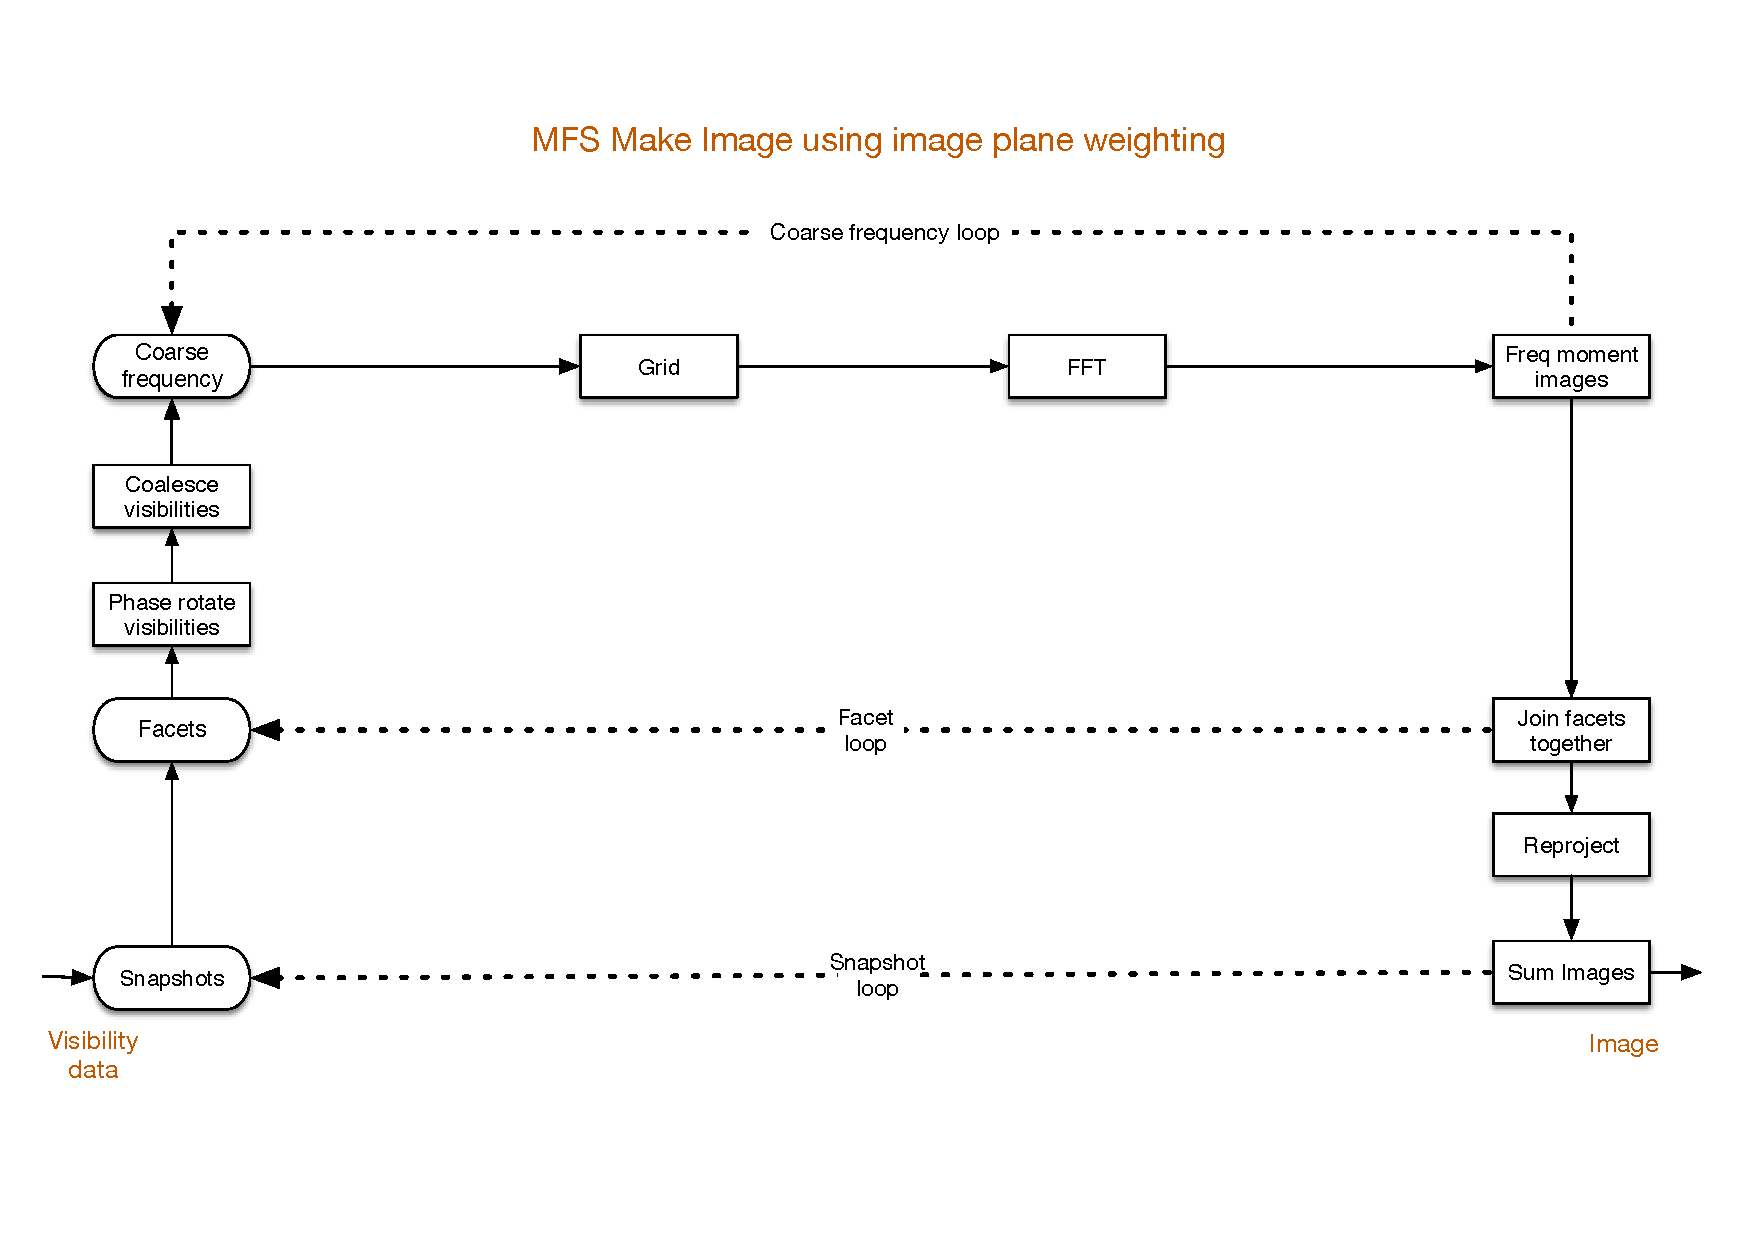
\includegraphics[width=\textwidth]{./MSMFS_MakeImage_Image.pdf}
  \caption{Structure of Image plane-weighting MakeImage, as used in CASA. Note that the three loops (denoted by the rectangle with curved ends) can be permuted at will.}
  \label{fig:makeimageimage}
\end{figure}

The CASA and ASKAPsoft approaches should be equivalent apart from numerical differences such as due to the convolution function. Hence either can be used according to the most favourable scaling. Compared to CASA, ASKAPsoft does approximately two orders of magnitude less FFTs and 5 times as much gridding. Both forms should therefore be available in the SDP Performance Model and used as the context dictates.

The Minor Cycle is identical in CASA and ASKAPsoft. The Minor cycle is depicted graphically in Figure \ref{fig:minor}.

\begin{figure}[htb]
  \centering
  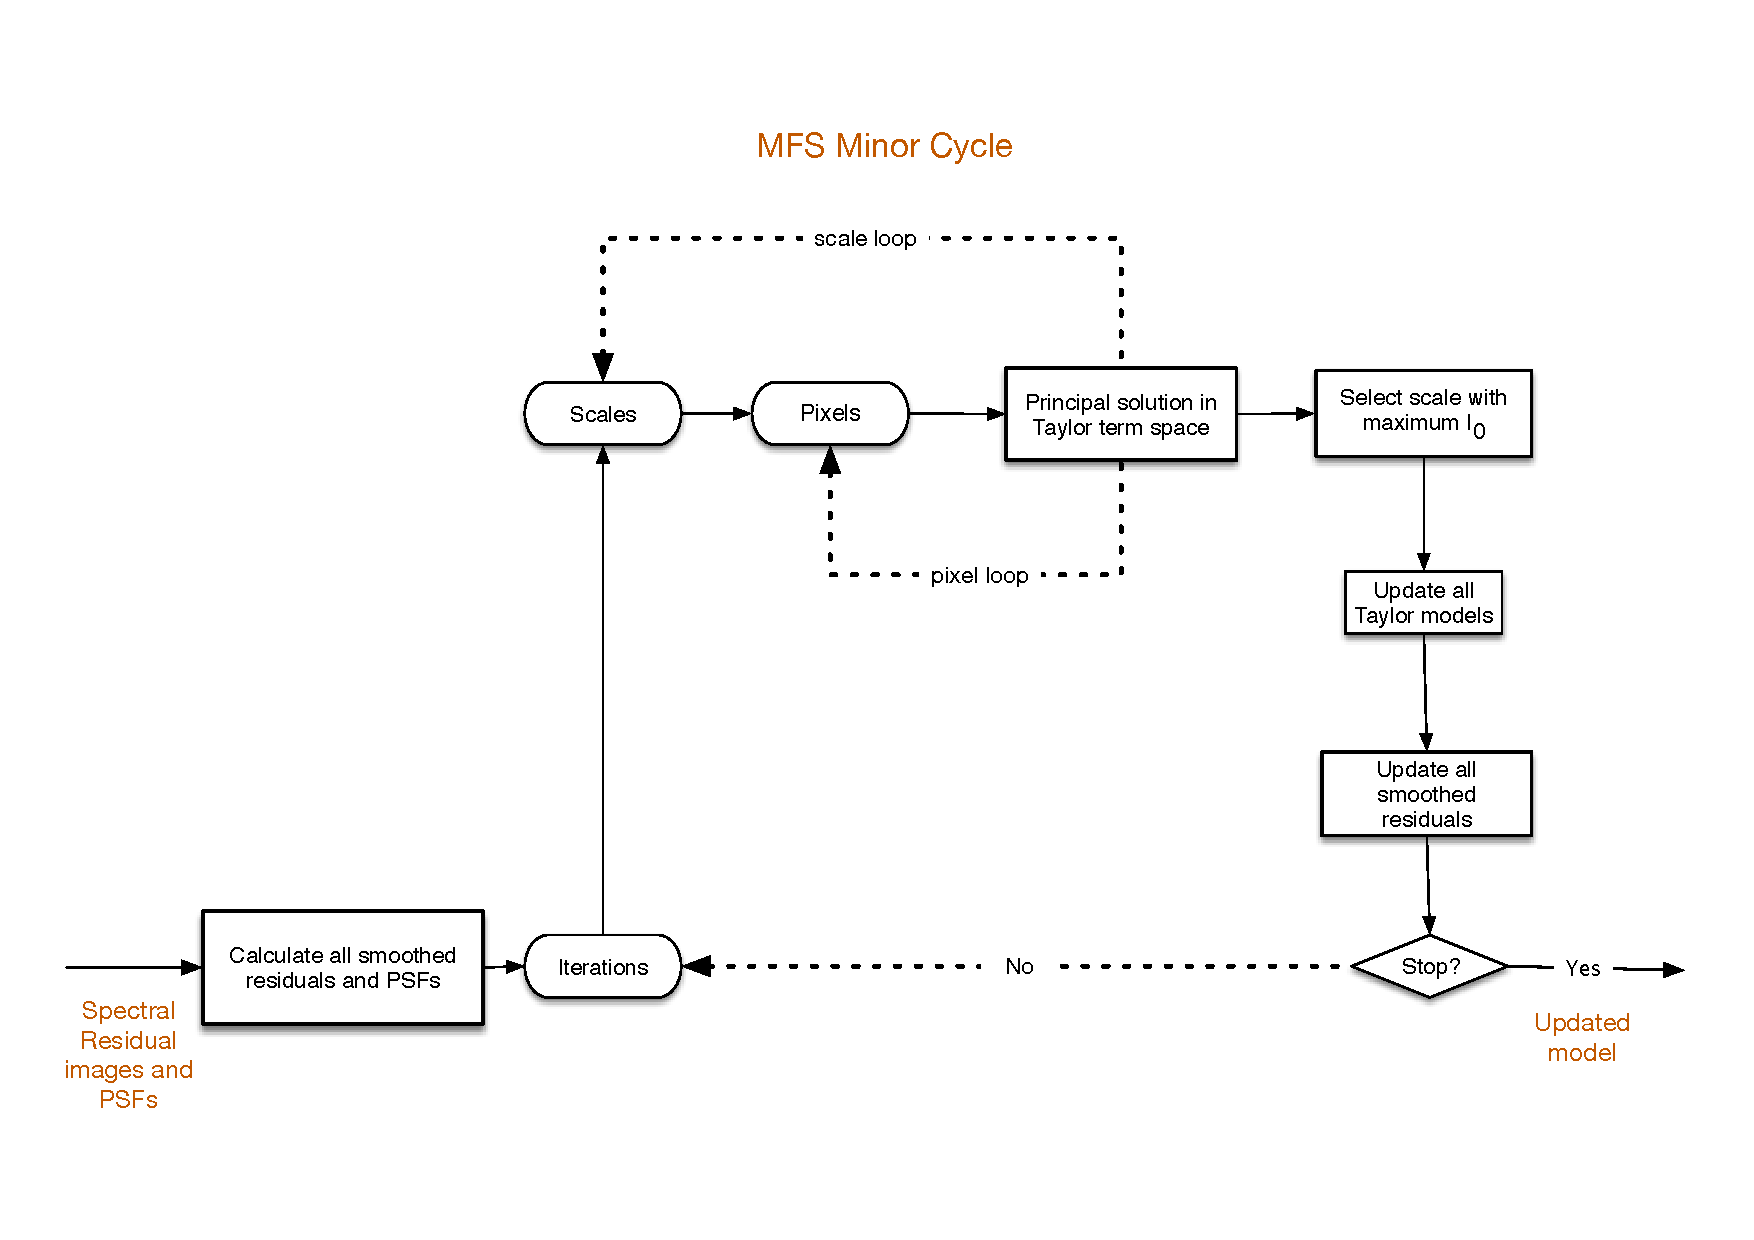
\includegraphics[width=\textwidth]{./MSMFS_Minor.pdf}
  \caption{Structure of Minor cycle for MSMFS as used in both CASA and ASKAPsoft.}
  \label{fig:minor}
\end{figure}


\clearpage
\section{Parallel processing}
\label{sec:parallel}

When moving the MSMFS algorithm to a distributed (loosely coupled) and parallel (tightly coupled) architecture such as the SDP architecture, there are a large number of important factors that must be considered.
\begin{description}
\item[Optimum partitioning] 
\item[Coupling across partitions] e.g. is the same pixel addressed in two different partitions? If so, is there a satisfactory approach to reconciling the two values?
\item[Synchronisation points] e.g. is a global synchronisation point required so that the deconvolutions can be made consistent? Is there an acceptable algorithm for reconciling separate facets?
\item[Amount of CU memory]
\item[Loading of CU memory backplane]
\item[Access to visibility store]
\end{description}

\subsection{Partitioning for Predict and MakeImage}
\label{subsec:partitoningpredictmakeimage}

The SDP pipeline framework [RD:??], allows partitioning across multiple axes. In this case, the natural partitions and typical values are:

\begin{description}
\item[Polarisation] Only Stokes I can be modelled using MSMFS
\item[Frequency] O(500) coarse channels are required to avoid bandwidth smearing
\item[Sub-bands] O(1-3) partitions of the coarse channels are required to ensure that the power law approximation is adequate.
\item[Time] O(43200) ~ O(1s) correlator samples are required to avoid smearing on the longest baselines
\item[Facet] O(100) facets to limit the size of the AW projection kernel
%\item[Snapshot time] O(100s) long gridding/degridding sequences are required to limit smearing due to w-plane rotation
\item[Scales] O(5) scales are typically required to model extended structure
\item[Taylor terms] O(5) terms are required to represent the spectral behaviour
\end{description}

According to the logic of the MSMFS algorithm, Sub-bands can be defined as the limit of the power law approximation for brightness so consequently can always be used as the coarsest partition. For Predict and MakeImage the remaining choices are as shown in Figure \ref{tab:partitions} (most rapid first):

\begin{table}[htp]
 \caption{Possible ordering of partitions $UV$ weighting version of Predict and MakeImage}
 \label{tab:partitions}
 \begin{center}
 \begin{tabular}{|c|c|c|c|}
\hline
Frequency & Time & Facet & Sub-Band \\
Frequency & Facet & Time & Sub-Band \\
Time & Facet & Frequency & Sub-Band \\
Time & Frequency & Facet & Sub-Band \\
Facet & Time & Frequency & Sub-Band \\
Facet & Frequency & Time & Sub-Band \\
\hline
\end{tabular}
\end{center}
\end{table}

The only choice is between the two orderings of Time and Facet. Since deconvolution is non-linear, we prefer that all times be represented in a single facet rather than the other way around.

Hence according to this level of analysis, the best ordering is [Frequency, Time, Facet, Sub-Band]. Parallelisation over Compute Nodes starts from the left to the right, Distribution over Compute Islands works from the right to the left (see Figure \ref{fig:order}):

\begin{figure}[htb]
  \centering
  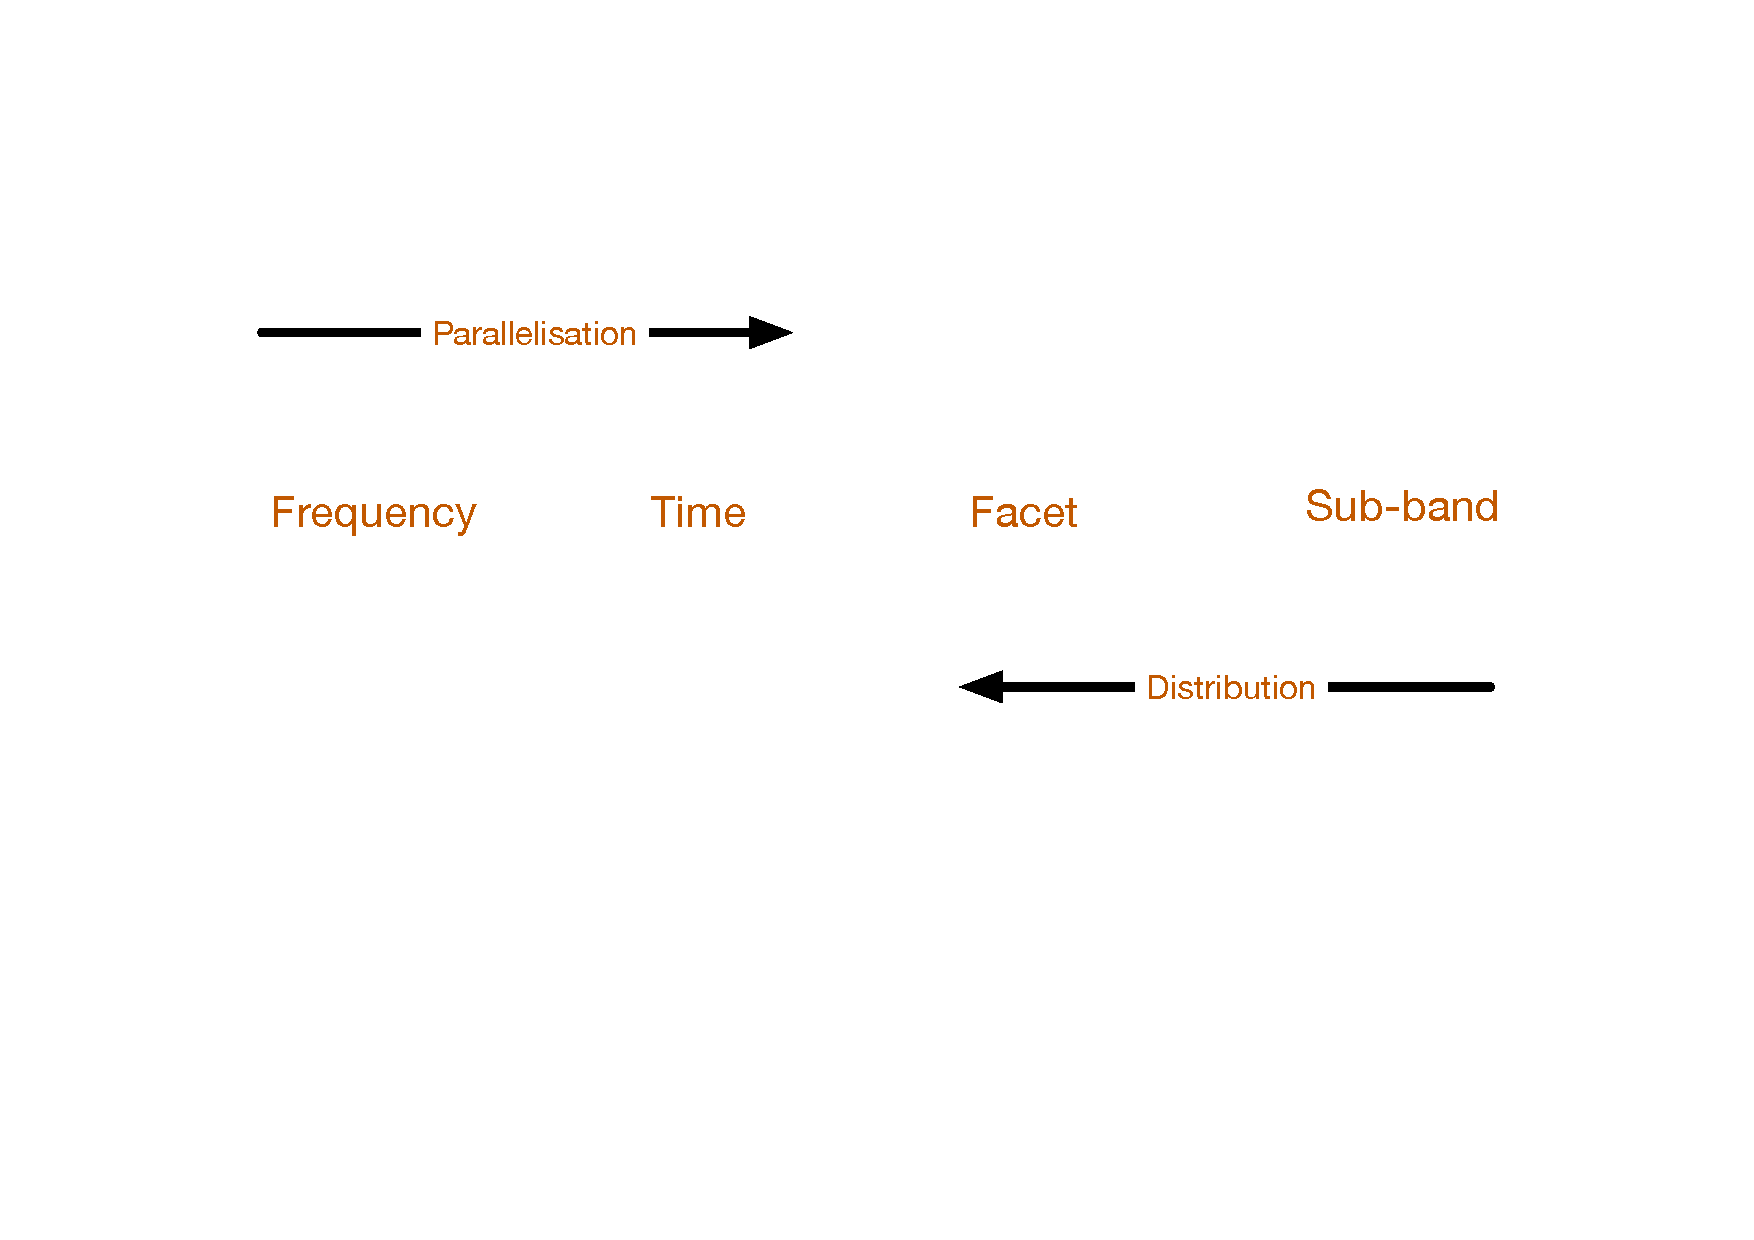
\includegraphics[width=\textwidth]{./Order.pdf}
  \caption{Preferred order of parallelisation and distribution for MakeImage and Predict sub-pipelines.}
  \label{fig:order}
\end{figure}

In this approach, the facets will almost certainly be processed on different compute islands. Note we have a dilemma on how to deal with the deconvolution of the facets.

\begin{itemize}	
\item Construct the facets with some padding, deconvolve each separately, and reconcile after deconvolution by facet to facet broadcast.
\item Construct the facets without padding, send all facets to one compute island, perform deconvolution, distribute models to facets. 
\end{itemize}

The first approach will inevitably introduce edge effects in the final image revealing the facet grid, while the second will block processing while deconvolution proceeds on the different sub-band compute nodes. We would then benefit from two different types of nodes:
\begin{description}
\item[Predict and MakeImage] Requires the visibility data but not many scratch images. Stalled during MinorCycle.
\item[MinorCycle] Requires a substantial number of scratch images, but not the visibility data. Stalled during Predict and MakeImage.	
\end{description}


\subsection{Partitioning for Minor Cycle}

In the minor cycle, the first calculation is [Pixel, Taylor Term], and then the Scale convolutions are calculated. Hence the natural order overall is [Pixel, Taylor Term, Scale]. This is used in both CASA and ASKAPsoft. Both use a single threaded Minor Cycle. For SDP, a multi-threaded but not-distributed Minor Cycle should be prototyped.

We have a modelling problem that is not going to be wished away. The science demands seamless imaging in multiple axes, whereas computing would like to partition the image cube in those same axes. There is a tendency to assert that one axis or another does not have to be seamless but that has not be conclusively argued. Distributing the minor cycle across Compute Islands may be possible in some cases (e.g. spectral line after continuum estimation and subtraction), but we should also be considering how best to parallelise the Minor Cycle on a single, appropriately specified Compute Island.

\subsection{Implementation in CASA}

The CASA tclean program supports parallel execution using python to run copies on different nodes. The visibility data are partitioned in time across the available processors. Gridding and transforms (i.e. Predict and MakeImage) are done separately and in parallel per partition. Then the Images (and weights) are gathered and then normalised. A serial minor cycle is run, blocking all other processing, and then the model image is scattered to all processes. The Major cycle is done in parallel per partition.

Thus in summary, the Major Cycles are parallelised while the deconvolution runs serially.

\subsection{Implementation in ASKAPsoft}

The ASKAPsoft code is mirrored in the SDP Github repository. The ASKAPsoft cimager is an MPI-enabled program. Since it was written as parallel program from the beginning, the structure is easier to follow than the CASA version. Distribution over MPI is via frequency, rather than time as in CASA. Predict and MakeImage are distributed using MPI (via a thin bookkeeping layer). The MinorCycle is performed on the master, and thus blocks until the deconvolution steps have completed.

The minor cycle  algorithm is in C++ Template DeconvolverMultiTermBasisFunction.tcc. The basis function is abstracted and can be any class having the interface DeconvolverMultiTermBasisFunction. There are two forms present: one for point sources, and one for the same blobs used in CASA - a truncated upside down parabola. The basis functions may optionally be orthogonalised using the Gramm-Schmidt algorithm.

The optimum blob location and scale is found by using one of two criteria:

\begin{description}
\item[MAXBASE0] The peak of term 0 across after decoupling in term.
\item[MAXCHISQ] The peak of chisquared across scale after decoupling in term.
\end{description}

The second criterion is expensive to compute and usually MAXBASE0 is used. Thus for each scale and for each pixel the pixel value at the reference frequency has to be determined by pre-multipling by the inverse Hessian (in term-term space). This means that the cost of the search is:

\begin{equation}
Rflop_{MSMFSminor} = N_{minor} N_{pix}^2 N_s N_T	
\end{equation}


To save on calculation, a number of cached images are used. For ASKAPsoft, these are shown in Table \ref{tab:askapmemory}.

\begin{table}[tbh]
\caption{ASKAPsoft cimager use of memory during minor cycles}\label{tab:askapmemory}

\begin{tabular}{|l|c|c|c|}
\hline
Item & Axes & Size (words) & Needed? \\
\hline
Basis function FFT & scales & $N_{pix} N_S $ & During initialisation \\
PSF FFT & 2 * Taylor terms & $2 N_{pix} N_T $ & During initialisation \\
Spectral Dirty image & Taylor terms, scales & $N_{pix} N_T N_s$ & During iteration \\
Spectral Dirty PSF & Taylor terms, scales & $N_{patch} N_T N_s$ & During iteration \\
Spectral Model image & Taylor terms & $N_{pix} N_T $ & During iteration \\	
Basis functions & scales & $N_{pix} N_s$ & During iteration \\
Inverse of Hessian & Taylor terms, Taylor terms, scales & $N^2_T N_s$ & During Iteration \\
\hline
\end{tabular}	
\end{table}

where $N_{pix}$ is the number of pixels in an image, $N_{patch}$ is the number of pixels in the patch of the Dirty beam used, $N_T$ is the number of Taylor terms, and $N_S$ is the number of scales/basis functions.

Thus, keeping only the dominant terms, the total memory used during iteration is: 

\begin{equation}
M_{MSMFS} = (N_T (N_s + 1) + N_s) N_{pix} 
\end{equation}

Using typical values of $N_t=5$ and $N_s=5$, we find that the memory use is about $35 N_{pix}$. For a 200,000 by 200,000 pixel image, this requires 5.6 TB total. Spread over O(100) Compute Islands (partitioning by facet and sub-band), this requires 56 GB per CI.



\clearpage
\section{A projection}
\label{sec:minor}

\clearpage
\section{Wide-band behaviour}
\label{sec:wideband}

\begin{itemize}
\item Does naive broadband work?
\item Bhatnagar et al WB algorithm	
\end{itemize}


\clearpage
\section{Recommendations}
\label{sec:recommendations}

\begin{enumerate}
\item Implement both Image and Visibility based calculation of the Taylor term images in the Performance Model.
\item Update the Performance Model to reflect the memory usage:
\begin{equation}
M_{MSMFS} = (N_T (N_s + 1) + N_s) N_{pix} 
\end{equation}
\item A multi-threaded Minor Cycle on one Compute Island should be prototyped.
\end{enumerate}



% \label{section:main}



% Add the bibliography
\clearpage \addcontentsline{toc}{section}{References}
\bibliography{your_bibfile}%



\end{document}

%%% Local Variables: 
%%% mode: latex
%%% TeX-master: t
%%% End: 
